\chapter{微积分学基本定理}
在前两章中,我们分别引入了函数的变率(导数),函数的和(定积分)的基本概念,本章将研究函数的导函数与函数的求和函数这两者之间的互逆关系,并说明我们可以用求导函数的逆运算方法来计算定积分.

\section{微积分学基本定理}
\subsection{导函数与求和函数}
函数$f(x)$在点$x_0$处的变化率(导数)的定义是
\[f' (x_0) =\lim_{h\to 0}\frac{f (x_0+h) -f (x_0)}{h}\]
显然, $f'(x_0)$的值与$f(x)$在点$x_0$的值以及在点$x_0$的邻近的函数值有关,当点$x_0$在$(a,b)$内变化时,$f'(x_0)$也跟着变化,那么$f'(x_0)$便是一个新函数称为$f(x)$的导函数.计算一个函数的导函数是一件比较简便的事情.

定积分$\int^b_a f(x)\dif x$的定义是把区间$[a,b]$无限细分
而得到上下夹逼阶梯函数的和的共同极限,其几何意义是曲线$y=f(x)$和直线$x=a$, $x=b$, 及$y=0$所围成的区域的有号面积.

假如我们考虑$f(x)$在一个变动的区间$[a,x]$上的和,
即让区间的左端点固定,右端点变动,则
\[S_f(x)=\text{函数$f$从$a$到$x$的和}=\int^x_a f (x) \dif x\]
可以看作上限变量$x$的函数,在这里,积分符号中的$x$既表示积分变量,又表示积分上限,容易混淆,因此,为了区别起见,我们用字母$t$来代表积分变量,这样上式就写成
\[S_f (x)=\int^x_a f(t)\dif t\]

和函数$S_f(x)$在$x=x_0$处的值$S_f(x_0)$的几何意义就是曲线$y=f(t)$, 直线$t=a$, $t=x_0$, $y=0$所围成的区域的有号面积,它是随区域的变动界线$t=x_0$的变动而变动的(图4.1).

\begin{figure}[htp]
    \centering
    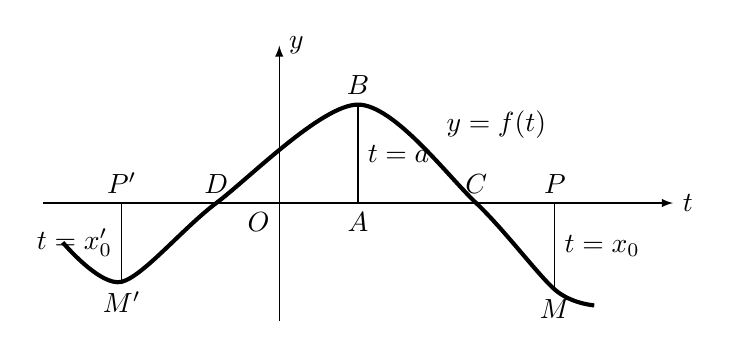
\begin{tikzpicture}[>=latex]
        \draw[->](-3,0)--(5,0)node[right]{$t$};
        \draw[->](0,-1.5)--(0,2)node[right]{$y$};
    \node at (0,0) [below left]{$O$};
    \node at (0,0){};
        \draw[line width=1.5pt] plot[smooth] coordinates{ (-2.75,-.5)(-2,-1)(-.8,0)(1,1.25)(2.5,0)(3.5,-1.1)(4,-1.3) 
    };
    \draw(-2,-1)node[below]{$M'$}--node[left]{$t=x_0'$}(-2,0)node[above]{$P'$};
    \draw(1,1.25)node[above]{$B$}--node[right]{$t=a$}(1,0)node[below]{$A$};
    \draw(3.5,-1.1)node[below]{$M$}--node[right]{$t=x_0$}(3.5,0)node[above]{$P$};
    \node at (-.8,0)[above]{$D$};
    \node at (2.5,0)[above]{$C$};
    \node at (2,1)[right]{$y=f(t)$};
    
    \end{tikzpicture}
    \caption{}
\end{figure}

例如,当变动界限(积分上限)在图中的$PM$位置时,则
\[S_f(x_0)=\int^{x_0}_a f(t)\dif t=ACB\text{的面积}-CPM\text{的面积}\]

当变动界限在图中的$P'M'$位置时,则
\[\begin{split}
    S_f(x'_0)&=\int^{x_0'}_a f(t)\dif t=-\int^a_{x_0'} f(t)\dif t\\
    &=-\left\{-P'DM'\text{的面积}+DAB\text{的面积}  \right\}\\
    &=P'DM'\text{的面积}-DAB\text{的面积}
\end{split}\]

例如,折线函数
\[g(x)=\begin{cases}
    \frac{1}{2}(x-1) & x\in[1,2]\\
    \frac{3}{2}(x-2)+\frac{1}{2}(2-1) & x\in [2,3]\\
    (x-3)+\frac{1}{2}(2-1)+\frac{3}{2}(3-2) & x\in [3,4]
\end{cases}\]
的导函数(除去在折线段的那些交接点处不作定义外)是阶梯函数
\[g'(x)=\begin{cases}
    \frac{1}{2} & x\in [1,2)\\
    \frac{3}{2} & x\in (2,3)\\
    1& x\in (3,4]
\end{cases}\]
反过来,该阶梯函数的和函数,是上述折线函数$g(x)$, 我们有如下的图解关系:
\begin{center}
    \begin{tikzpicture}[>=latex]
        \node (A) at (0,0) {\{折线函数\}};
        \node (B) at (5,0) {\{阶梯函数\}};
\draw[->](A) to [bend left=30]node[above]{求导} (B);
\draw[->](B) to [bend left=30]node[above]{求和} (A);

    \end{tikzpicture}
\end{center}

上述简明的例子表明“微分”与“积分”(或求函数由$a$到$b$的和)之间的运算关系应该是互逆的.

\subsection{微积分学基本定理}

\begin{blk}
  {定理1} 设$f(t)$是在$[a,b]$上的分段单调连续函数,又它的和函数是
\[S_f(x)=\int^x_a f (t) \dif t\]
那么
\[\frac{\dif }{\dif x}S_f(x)=\frac{\dif }{\dif x}\int^x_a f (t) \dif t=f(x),\qquad a\le x\le b\]
\end{blk}

\begin{figure}[htp]
    \centering
    \begin{tikzpicture}[>=latex, xscale=3]
        \draw[->](.4,0)--(3,0)node[right]{$t$};
        \draw[->](.6,-.5)--(.6,4.5)node[right]{$y$};
    \draw[domain=.9:2.5, very thick, samples=100]plot(\x, {2.5*(\x-1)*(\x-2)*(\x-3)+2})node[right]{$y=f(t)$};
    \draw(.9,0)node[below]{$a$}--(.9,1.4225);
    \draw[pattern=north east lines, domain=1.4:1.7, samples=50]plot(\x, {2.5*(\x-1)*(\x-2)*(\x-3)+2})--(1.7,2.6825)--(1.7,0)node[below]{$x$}--(1.4,0)node[below]{$x+\bar h$}--(1.4,2.96);
    \draw[pattern=north west lines, domain=1.7:2, samples=50]plot(\x, {2.5*(\x-1)*(\x-2)*(\x-3)+2})--(2,2)--(2,0)node[below]{$x+h$}--(1.7,0)--(1.7,2.6825);
    \draw[<-](1.55,2)--(1.55,3.5)node[right]{$S_f(x)-S_f(x+\bar h),\; (\bar h<0)$};
    \draw[<-](1.85,.5)--(2.1,.5)node[right]{$S_f(x+h)-S_f(x),\; (h>0)$};
    \node at (.6,0)[below left]{$O$};
    \end{tikzpicture}
    \caption{}
\end{figure}

\begin{proof}
  如图4.2,设$h>2$,则
\[\begin{split}
    \frac{S_f(x+h)-S_f(x)}{h}&=\frac{\Int^{x+h}_a f(t)\dd t-\Int^{x}_a f(t)\dd t}{h}\\
    &=\frac{\Int^{x+h}_x f(t)\dd t}{h}\qquad \text{(定积分性质1)}\\
    &=\frac{hf(\xi)}{h}\quad (x<\xi<x+h)\\
    &=f(\xi)\qquad \text{(定积分中值定理)}
\end{split}\]
于是
\begin{equation}
    \lim_{h\to 0^+}\frac{S_f(x+h)-S_f(x)}{h}=\lim_{\xi\to x}f(\xi)=f(x)
\end{equation}

设$\bar h<0$,则
\[\begin{split}
    \frac{S_f(x)-S_f(x+\bar h)}{\bar h}&=\frac{\Int^{x}_a f(t)\dd t-\Int^{x+\bar h}_a f(t)\dd t}{\bar h}\\
    &=\frac{\Int^{x}_{x+\bar h} f(t)\dd t}{\bar h}\qquad \text{(定积分性质1)}\\
    &=\frac{-\bar h f(\bar\xi)}{\bar h}=-f(\bar\xi)\quad (x+\bar h<\bar \xi<x)\\
\end{split}\]
即:
\[\frac{S_f(x+\bar h)-S_f(x)}{\bar h}=f(\bar\xi),\qquad (x+\bar h<\bar \xi<x)\]
于是
\begin{equation}
    \lim_{h\to 0^-}\frac{S_f(x+\bar h)-S_f(x)}{\bar h}=\lim_{\bar\xi\to x}f(\bar\xi)=f(x)
\end{equation}
由(4.1)和(4.2),得
\[\frac{\dd }{\dd x}S_f(x)=\frac{\dd }{\dd x}\int^x_a f(t)\dd t=f(x)\]
\end{proof}

\begin{blk}
    {引理} 如果两个函数$F(x)$和$G(x)$满足条件
\[F' (x) =G' (x) ,\qquad a\le x\le b\]
那么
\[G(x)=F(x)+C,\qquad (C\text{是常数})\]
\end{blk}

\begin{proof}
    由$G'(x)-F'(x)=0$, 得
\[[G (x) -F (x) ]'=0\]
根据中值定理(参看第三章)知,对于每一个$x\in (a,b)$, 恒有
\[G(x)-F(x)=C,\qquad (C\text{是常数})\]
所以
\[G (x) =F (x) +C\]
\end{proof}

\begin{blk}
 {定义} 设$f(x)$是在区间$[a,b]$上给定的函数,如果可微函数$G(x)$满足条件
\[G'(x)=f(x)\qquad (\text{或}\quad \dd G(x)=f(x)\dd x)\]
那么就称$G(x)$为$f(x)$在$[a,b]$上的一个\textbf{原函数}.
\end{blk}

例如,设$G'(x)=\cos x$, 那么$G(x)=\sin x$就称为$\cos x$的一个原函数.

\begin{blk}
    {定理2} 设$f(x)$是给定的分段单调连续函数,如果一个可微函数$G(x)$满足条件
\begin{equation}
    G'(x)=f(x)\qquad \text{(或$\dd G(x)=f(x)\dd x$)},\quad a\le x\le b
\end{equation}    
那么
\[S_f (x)=\int^x_a  f (t) \dd t=G (x) -G (a) \]
\end{blk}

\begin{proof}
    由定理1知,$f(x)$的一个原函数存在,就是它的和函数,即
\[\frac{\dd }{\dd x}\int^x_a f(t)\dd t=f(x)\]
题设$G(x)$是$f(x)$的另一个原函数,故由引理得
\begin{equation}
    \int^x_a    f (t) dt=G (x) +C 
\end{equation}
这里的常数要由条件$\Int^a_a f(t)\dd t=0$来确定.

在(4.4)中,令$x=a$,得
\[0=G(a)+C\]
所以:$C=-G(a)$,代入(4.4),得
\[\int^x_a f(t)\dd t=G(x)-G(a)\]
\end{proof}

在上面等式中,令$x=b$, 便得到下面著名的莱布尼兹-牛顿公式:
\[\int^b_a f (t) \dd t= G (b) -G (a) \]
这个公式告诉我们,求分段单调连续函数$f(x)$在$[a,b]$上的定积分可以化简为去求$f(x)$的一个原函数$G(x)$, 而函数值的差$G(b)-G(a)$就是定积分的值.

\begin{example}
    设$f(x)=k$(常数函数),则$G(x)=kx$是一个满足$G'(x)=k=f(x)$的原函数,所以
\[\int^b_a k\dd x=kb-ka=k(b-a)\]
以后我们引用一个符号:
\[G(x)\Bigg|^b_a=G(b)-G(a)\]
\end{example}

\begin{example}
    设$f(x)=kx^n,\; (n\in\mathbb{N})$,则
\[G(x)=k\frac{x^{n+1}}{n+1}\]
是满足$G'(x)=kx^n$的一个原函数,所以
\[\int^b_akx^n\dd x=k\frac{x^{n+1}}{n+1}\Bigg|^b_a=\frac{k}{n+1}(b^{n+1}-a^{n+1})\]
\end{example}

\begin{example}
设$f(x)=x^{-n}=\frac{1}{x^n}\; (x\ne 0,\; n\in\mathbb{N})$,则
\[G(x)=\frac{x^{-n+1}}{-n+1}\]
是满足$G'(x)=x^{-n}$的一个原函数.要特别注意定理2中$f(x)$是连续的条件,在任何包含0的区间上,函数$f(x)=\frac{1}{x^n}$无界,即有第二类间断点,如果$a,b$异号,则定积分$\Int^b_a x^{-n}\dd x$无意义,但若$a,b$同时为正或同时为负,则
\[\int^b_ax^{-n}\dd x=\frac{x^{-n+1}}{-n+1}\Bigg|^b_a=\frac{b^{-n+1}}{-n+1}-\frac{a^{-n+1}}{-n+1}\]
当然,又有$n\ne -1$时,上式才能成立.

如果$n=-1$,依复合函数求导法则,得
\[(\ln|x|)'=\frac{1}{|x|}\cdot |x|'\]
若$x>0$,则
\[(\ln|x|)'=\frac{1}{x}\cdot 1=\frac{1}{x}\]
若$x<0$,则
\[(\ln|x|)'=\frac{1}{-x}\cdot (-1)=\frac{1}{x}\]
总之
\[(\ln|x|)'=\frac{1}{x},\quad (x\ne 0)\]
因此
\[\begin{split}
\int^b_a \frac{1}{x}\dd x=\ln |x|\Bigg|^b_a &=\ln|b|-\ln |a|\\
&=\ln\left|\frac{b}{a}\right|=\ln\frac{b}{a}\quad (x\ne 0,\; ab>0)
\end{split}\]
\end{example}

\begin{example}
    求$\Int^3_1 |x-2|\dd x$
\end{example}

\begin{solution}
\[\begin{split}
    \Int^3_1 |x-2|\dd x&=\Int^2_1 -(x-2)\dd x+\Int^3_2 (x-2)\dd x\\
&=\left(-\frac{x^2}{2}+2x\right)\Bigg|^2_1+\left(\frac{x^2}{2}-2x\right)\Bigg|^3_2\\
&=\frac{1}{2}+\frac{1}{2}=1
\end{split}\]
\end{solution}

\begin{example}
求$\Lim_{n\to\infty}\frac{\sum^n_{i=1}i^p}{n^{p+1}}\quad (p\in \mathbb{N})$
\end{example}


\begin{solution}
\[\begin{split}
    \Lim_{n\to\infty}\frac{\sum^n_{i=1}i^p}{n^{p+1}}&=\Lim_{n\to\infty}\sum^n_{i=1}\left(\frac{i}{n}\right)^p\cdot \frac{1}{n}\\
    &=\int^1_0 x^p\dd x=\left.\frac{x^{p+1}}{p+1}\right|^1_0=\frac{1}{p+1}
\end{split}\]
\end{solution}

\begin{ex}
\begin{enumerate}
\item 用求原函数的方法, 计算下列定积分:
\begin{multicols}{2}
\begin{enumerate}
 \item $\Int_{2}^{3}\left(x^{3}+6 x^{2}+4 x+1\right) \dd x$
\item $\Int_{1}^{5} \frac{v^{2}+2}{v^{4}} \dd v$
\item $\Int_{-3}^{-2}\left(x+\frac{2}{x}\right)^{2} \dd x$
\item $\Int_{1}^{10}\left(x+\frac{1}{x}\right) \dd x$
\item $\Int_{a}^{b}|x-1| \dd x$
\end{enumerate}
\end{multicols}
\item 求曲线 $y=2 x-x^{2}$ 与 $x$ 轴之间的面积.
\item 设 $y=x(x-1)(x-2)$,
求 $\Int_{0}^{1} y \dd x,\; \Int_{1}^{2} y\dd x,\; \Int_{0}^{2} y \dd x$,
并说明所得结果的几何意义.

\item 求直线$y=2x$和曲线$y=x^2$之间的面积.
\item 求由曲线$y=\frac{1}{x^2}$和直线$x=1$, $x=4$所围成的曲边梯形的
面积.
\item 求抛物线方程使它具有以下的性质:
\begin{enumerate}
\item 抛物线通过$(0, 0)$, $(1, 2)$两点,
\item 它的对称轴平行$y$轴,且向上凸,
\item 它与$x$轴所围的面积最小.
\end{enumerate}

\item 求正数$a$, 使$\Int^1_0 |x^2-a^2|\dd x$最小.
\item 求下列函数的导数:
\begin{multicols}{2}
    \begin{enumerate}
     \item $F(x)=\Int_{a}^{x}\sin^2 t \dd t$
    \item $F(x)=\Int_{a}^{x^2} \sin^2 t \dd t$
    \end{enumerate}
    \end{multicols}
\end{enumerate}

\end{ex}

\section{不定积分}
由上节的微积分基本定理得知,在$[a,b]$上的两个可
微函数$G_1(x)$和$G_2(x)$均以$f(x)$为其导数,则$G_1(x)$与$G_2(x)$在$[a,b]$上只差一个常数$C$. 由此可见,如果$G'(x)=f(x)$, 且$C$为任意常数,那么$[G(x)+C]'=G'(x)=f(x)$. 这就是说:如果 函数$f(x)$有一个原函数$G(x)$, 那么就有无穷多个原函数,并且所有原函数刚好组成函数族
\[\{G(x)+C\;|\; C\text{是任意常数}\}\]

\begin{blk}
   {定义} 函数$f(x)$在区间$[a,b]$上的原函数全体叫做$f(x)$的不定积分,记作
   \[\int f(x)\dd x\]
   设$G(x)$是$f(x)$的一个原函数,那么由不定积分的定义得到
\[\int f (x) \dd x=G (x) +C\]
   其中$C$是任意常数.
\end{blk}   

关于不定积分,易见有如下性质:

\begin{blk}{性质1}
   积分与微分互为逆运算,即:
\[\begin{cases}
    \dd\Int f(x)\dd x=f(x)\dd x\\
    \Int \dd f(x)=f(x)+C
\end{cases}\]
\end{blk}

事实上,因为$\frac{\dd }{\dd x}\Int^x_a f(t)\dd t=f(x)$,所以
\[\int f(x)\dd x=\int^x_a f(t)\dd t+C\qquad \text{(基本定理1和不定积分定义)}\]
于是
\[\left(\int f(x)\dd x\right)'=\left(\int^x_a f(x)\dd x\right)'=f(x)\]
从而
\[\dd\int f(x)\dd x=f(x)\dd x\]
又
\[\begin{split}
    \int \dd f(x)&=\int f'(x)\dd x=\int^x_a f'(t)\dd t+C_1\\
    &=f(x)-f(a)+C_1\quad \text{(基本定理)}\\
    &=f(x)+C
\end{split}\]
这里$C=-f(a)+C_1$. 

从性质1看出,若不要不定积分等式中的任意常数项,则当符号$\Int$与$\dd$紧接着时,无论哪个在前,哪个在后,都可以消掉.

因为微分,积分是两种互逆的运算,所以它们的运算法则是互相对应的,现将它们相对应的法则叙述如下:

\begin{blk}{性质2}
 \[\begin{cases}
     {\rm d} [f(x)+g(x)]=\dd f(x)+\dd g(x)\\
     \Int [f(x)+g(x)] \dd x=\Int f(x)\dd x+\Int g(x)\dd x+C
 \end{cases}\]
 \end{blk}

 上面不定积分公式的正确性不难证明,只要求出两边的微商,由于所得到的微商恒等,就可以知道它们只差一个常数项,因为,由性质1
\[\begin{split}
    \left(\int[f(x)+g(x)]\dd x\right)'&=f(x)+g(x)\\
    \left(\int f(x)\dd x+\int g(x)\dd x\right)'&=\left(\int f(x)\dd x\right)'+\left(\int g(x)\dd x\right)'=f(x)+g(x)
\end{split}\]
所以$f(x)+g(x)$的两个原函数相差一个常数项,即:
\[\int[f(x)+g(x)]\dd x=\int f(x)\dd x+\int g(x)\dd x+C\]
同理可得:

\begin{blk}{性质3}
\[\begin{cases}
    {\rm d} [a f(x)]=a\dd f(x)\\
    \Int af(x)\dd x=a\Int f(x)\dd x
\end{cases}\qquad (a\ne 0)\]
\end{blk}

\subsection{基本积分表}

由基本微商公式表,倒转顺序,就可以得到下面这个表:
\begin{itemize}
    \item $\frac{\dd}{\dd x}C=0,\qquad \Int 0\dd x=C$
    \item $\frac{\dd }{\dd x}x^{\mu}=\mu x^{\mu-1},\qquad \Int x^{\mu}\dd x=\frac{x^{\mu+1}}{\mu+1}+C\quad \text{($\mu$是不等于$-1$的实数)}$
    \item $\frac{\dd }{\dd x}\ln|x|=\frac{1}{x},\qquad \Int\frac{\dd x}{x}=\ln|x|+C\quad (x\ne 0)$
    \item $\frac{\dd }{\dd x}e^x=e^x,\qquad \Int e^x\dd x=e^x+C$
\end{itemize}
还因为$a^x=e^{x\ln a}$,由复合函数求导法则,得:
\[(a^x)'=e^{x\ln a}(x\ln a)'=\ln a\cdot e^{x\ln a}=\ln a\cdot a^x\]
所以:
\begin{itemize}
    \item $\frac{\dd}{\dd x}a^x=\ln a\cdot a^x,\qquad \Int a^x\dd x=\frac{a^x}{\ln a}+C$
    \item $\frac{\dd}{\dd x} \sin x=\cos x, \qquad \Int \cos x \dd x=\sin x+C$.
    \item $\frac{\dd}{\dd x} \cos x=-\sin x, \qquad \Int \sin x \dd x=-\cos x+C$.
    \item  $\frac{\dd}{\dd x}\tan  x=\sec ^{2} x, \qquad \Int \sec^{2} x \dd x=\tan x+C$
    \item $\frac{\dd}{\dd x}\cot x=-\csc ^{2} x, \qquad \Int \csc^{2} x \dd x=-\cot x+C$
    \item $\frac{\dd}{\dd x} \arcsin x=\frac{1}{\sqrt{1-x^{2}}} ,\qquad \Int \frac{\dd x}{\sqrt{1-x^{2}}}=\arcsin x+C$ 
    
    $\frac{\dd}{\dd x} \arccos x=\frac{-1}{\sqrt{1-x^{2}}},\qquad \Int\frac{-1}{\sqrt{1-x^{2}}}\dd x=-\arccos x+C'$
    \item  $\frac{\dd}{\dd x}\arctan x=\frac{1}{x^{2}+1}, \qquad \Int \frac{\dd x}{x^{2}+1}=\arctan x+C$ 
    
    $\frac{\dd}{\dd x} \arccot x=\frac{-1}{x^{2}+1}, \qquad \Int \frac{-1}{x^{2}+1}\dd x=-\arccot  x+C'$
\end{itemize}

现在来看不定积分的几何意义.

由不定积分的定义知道,求函数$f(x)=3x^2$的原函数全体,就是求不定积分$\Int 3x^2\dd x$, 也就是求满足微分方程
\begin{equation}
    \frac{\dd y}{\dd x}=3x^2
\end{equation}
的所有的原函数.

显然,$y=x^3$就是微分方程(4.5)的一个原函数,它的图象上各点切线的斜率由(4.5)确定.我们称曲线$y=x^3$为
微分方程(4.5)的积分曲线,把它沿$y$轴上下平移任意一段距离,便得到曲线族
\begin{equation}
    y=x^3+C
\end{equation}
并且(4.6)中任意一条曲线与曲线$y=x^3$在横坐标相同的点的切线平行,其斜率都等于$3x^2$, 因此,曲线族(4.6)是满足微分方程(4.5)的所有积分曲线,也就是不定积分$\Int 3x^2\dd x=x^3+C$的几何表示(图4.3).

为要确定(4.5)的某条积分曲线的位置,应当给出这条积分曲线必须经过的一点,例如它经过点$P(1, 3)$. 我们说这条件也是微分方程(4.5)的一个相应的原函数要满足的初值条件
$y\big|_{x=1}=3$
把它们代入(4.6), 得到
\[3=1^3+C\quad \Rightarrow\quad C=2\]
因此,满足微分方程$\frac{\dd y}{\dd x}=3x^2$和初值条$y\big|_{x=1}=3$的原函
数或相应的积分曲线是
\[y=x^3+2\]

通常把满足微分方程
\begin{equation}
\frac{\dd y}{\dd x}=f(x)
\end{equation}
的所有解叫做给定函数$f(x)$的不定积分,即
\[y=\int f(x)\dd x\]
把函数$f(x)$的一个原函数$y=G(x)$的图象叫做微分方程(4.7)的一条\textbf{积分曲线},这样,不定积分
\[y=\int f(x)\dd x=G(x)+C \quad \text{($C$为任意常数)}\]
的几何意义就表示与$y=G(x)$在各点有相同斜率$\frac{\dd y}{\dd x}=f(x)$的积分曲线族(图4.3).
\begin{figure}[htp]
    \centering
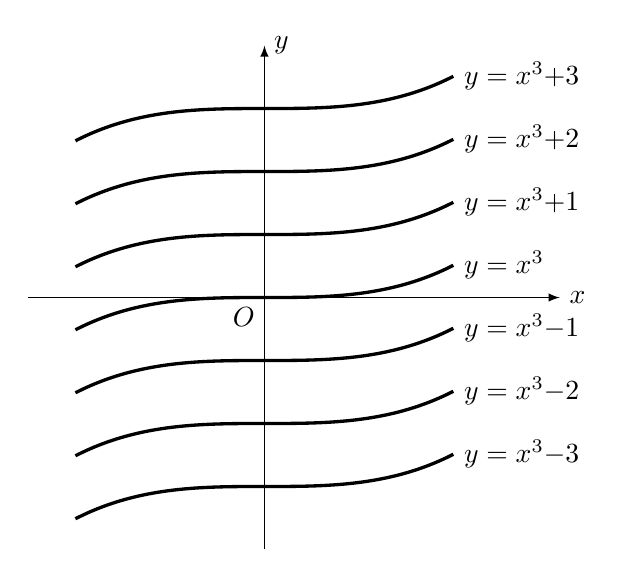
\begin{tikzpicture}[>=latex, xscale=3, yscale=.8]
\draw[->](-1,0)--(1.25,0)node[right]{$x$};
\draw[->](0,-4)--(0,4)node[right]{$y$};
\node at (0,0)[below left]{$O$};
\foreach \y in {1,2,3}
{
    \draw[domain=-.8:.8, samples=100, very thick]plot(\x, {\x*\x*\x+\y})node[right]{$y=x^3+$\y};
    \draw[domain=-.8:.8, samples=100, very thick]plot(\x, {\x*\x*\x-\y})node[right]{$y=x^3-$\y};
}
\draw[domain=-.8:.8, samples=100, very thick]plot(\x, {\x*\x*\x})node[right]{$y=x^3$};
\end{tikzpicture}
    \caption{}
\end{figure}

由微积分基本定理2知道,如果$y=G(x)$满足下面两个条件:
\[G'(x)=f(x)\quad \text{且}\quad G(a)=0\]
那么,$y=G(x)$就是$f(x)$的求和函数$G(x)=\Int^x_a f(x)\dd x$.

\begin{example}
求$\Int \sin (kx)\dd x,\quad \Int \cos(kx)\dd x,\quad \Int e^{kx}\dd x,\quad \Int \frac{\dd x}{x^2+a^2}$
\end{example}

\begin{solution}
    因为
\[\begin{split}
    (\cos kx)'&=-k\sin kx\\
    (\sin kx)'&=k\cos kx\\
    (e^{kx})'&=ke^{kx}\\
    \left(\arctan\frac{x}{a}\right)'&=\frac{1}{\left(\frac{x}{a}\right)^2+1}\cdot\left(\frac{x}{a}\right)'=\frac{a}{x^2+a^2}
\end{split}\]
所以
\[\begin{split}
    \int \sin (kx)\dd x&=-\frac{1}{k}\cos kx+C\\
    \Int \cos(kx)\dd x&=\frac{1}{k}\sin kx+C\\
    \Int e^{kx}\dd x&= \frac{1}{k}e^{kx}+C\\
    \Int \frac{\dd x}{x^2+a^2}&=\frac{1}{a}\arctan\frac{x}{a}+C \\
\end{split}  \]
\end{solution}

\begin{example}
    证明:若$\Int f(t)\dd t=F(t)+C$,则
\[\int f(kx)\dd x=\frac{1}{k}F(kx)+C\]
\end{example}

\begin{proof}
只须证明$f(kx)$的一个原函数是$\frac{1}{k}F(kx)$即可.
我们求$\frac{1}{k}F(kx)$对$x$的导数,于是
\[\frac{\dd}{\dd x}\left[\frac{1}{k}F(kx)\right]=\frac{1}{k}F'(kx)\cdot (kx)'=F'(kx)\]
由题设知$F' (t) =f (t)$, 所以
\[\frac{\dd}{\dd x}\left[\frac{1}{k}F(kx)\right]=F'(kx)=f(kx)\]
因此
\[\int f (kx) \dd x=\frac{1}{k}F (kx) +C\]
\end{proof}

\begin{example}
求$\Int \sin kx\sin\ell x\dd x$
\end{example}

\begin{solution}
\[\begin{split}
    \Int \sin kx\sin\ell x\dd x&=\int \frac{1}{2}[\cos(k-\ell)x-\cos(k+\ell)x]\dd x\\
    &=\frac{1}{2}\int \cos (k-\ell)x\dd x-\frac{1}{2}\int \cos (k+\ell)x\dd x\\
&=\frac{\sin(k-\ell)x}{2(k-\ell)}-\frac{\sin(k+\ell)x}{2(k+\ell)}+C
\end{split}\]
    这里$k\ne \pm \ell$.(如果$k=\pm\ell$,则另当考虑)
\end{solution}


\begin{example}
求$\Int \left(\frac{2a}{\sqrt{x}}-\frac{b}{x^2}+2xc^{\tfrac{2}{3}}\right)\dd x$
\end{example}


\begin{solution}
    \[\begin{split}
        \Int \left(\frac{2a}{\sqrt{x}}-\frac{b}{x^2}+2xc^{\tfrac{2}{3}}\right)\dd x&=2a\int x^{-\tfrac{1}{2}}\dd x-b\int x^{-2}\dd x+3c\int x^{\tfrac{2}{3}}\dd x\\
        &=4a\sqrt{x}+\frac{b}{x}+\frac{9}{5}cx^{\tfrac{5}{3}}+C
    \end{split}\]
\end{solution}

\begin{example}
    求$\Int \frac{3x^2}{1+x^2}\dd x$
\end{example}

\begin{solution}
\[\begin{split}
    \Int \frac{3x^2}{1+x^2}\dd x&=3\int \left(1-\frac{1}{x^2+1}\right)\dd x\\
    &=3\int \dd x-3\int \frac{\dd x}{x^2+1}\\
    &=3x-3\arctan x+C
\end{split}\]
\end{solution}

以上各例都是利用不定积分的性质2、3, 同时配合使用三角恒等式或设法将被积函数拆成几项,从而把一个比较复杂的积分化成若干个可以查基本积分表的积分.

\begin{ex}
\begin{enumerate}
    \item 计算下列不定积分:
\begin{multicols}{2}
\begin{enumerate}
\item  $\Int\left(x^{3}+3 x+5\right) \dd x$
\item  $\Int(x+2)^{4} \dd x$
\item  $\Int\left(x^{-2}+x^{-1}+x^{\tfrac{1}{3}}+x^{\tfrac{1}{2}}\right) \dd x$
\item  $\Int\left(a^{\tfrac{2}{3}}-x^{\tfrac{2}{3}}\right)^{3} \dd x$
\item  $\Int\left(\frac{1}{x}+e^{x}\right) \dd x$
\item  $\Int \frac{2 \cdot 3^{x}-5 \cdot 2^{x}}{3^{x}} \dd x$
\item  $\Int \left(\frac{3}{1+x^{2}}-\frac{2}{\sqrt{1-x^{2}}}\right) \dd x$
\item  $\Int \frac{2+x^{2}}{1+x^{2}} \dd x$
\item  $\Int \frac{\dd x}{x^{2}\left(1+x^{2}\right)}$
\item  $\Int \frac{\dd x}{x^{2}\left(a^{2}+x^{2}\right)}$
\item  $\Int 3^{x} e^{x} \dd x$
\end{enumerate}
\end{multicols}

\item  利用三角恒等式, 计算下列不定积分:
    \begin{multicols}{2}
        \begin{enumerate}
    \item  $\Int \tan^{2} x \dd x$
    \item  $\Int \frac{\cos 2 x}{\cos x-\sin x} \dd x$
    \item  $\Int \frac{2+\sin ^{2} x}{\cos ^{2} x} \dd x$
    \item  $\Int \sin ^{2} x \dd x$
    \item  $\Int \cos ^{2} x \dd x$
    \item  $\Int \cos k x \cos \ell x \dd x$
    \item  $\Int \sin 2 x \cos 5 x \dd x$
    \item  $\Int \frac{\dd t}{\sin ^{2} t \cos ^{2} t}$
    \item  $\Int \sin ^{3} x \dd x$
    \item  $\Int \cos ^{3} x \dd x$
\end{enumerate}
\end{multicols}    

\item 若$\Int f(t)\dd t=F(t)+C$, 求证
\[\int f (ax+b) \dd x=\frac{1}{a}F (ax+b) +C\]
\item  若$\frac{\dd y}{\dd x}=4x-6$, 且当$x=0$时,$y=9$, 求$y$的极小值.
\item  若$\frac{\dd y}{\dd x}=ax+b$, 求原函数$y=f(x)$使其满足下列条件:
\begin{enumerate}
    \item 当$x=0$时,$y=5$;
    \item 积分曲线向下凸且曲线$y=f(x)$在$x$轴上截得的弦长等于4;
    \item 曲线$y=f(x)$上纵坐标的最小值等于$-4$.
\end{enumerate}
\item 试求一个次数最低的多项式,使之当$x=1$时,有最大值6,而当$x=3$时,有最小值2.
\item  求下列各式的极限:
\begin{enumerate}
    \item $\Lim_{n\to\infty}\frac{\sqrt[n]{e}+\sqrt[n]{e^2}+\cdots+\sqrt[n]{e^n}}{n}$
    \item $\Lim_{n\to\infty}\frac{\sqrt[n]{e}+\sqrt[n]{e^4}+\cdots+\sqrt[n]{e^{2n}}}{n}$
\end{enumerate}
\end{enumerate}

\end{ex}


\section{不定积分的计算方法}
从上一节看到,虽然利用积分运算法则及基本积分表可以求出不少函数的原函数,但是实际遇到的积分仅凭这一些
方法还不能完全解决,本节将介绍几种典型的方法,利用这些方法,我们就可以计算更多的不定积分,此外,我们还制作了较为详细的积分表,可供使用时查阅.

\subsection{第一换元法}

有一些不定积分,将积分变量进行某种变映后就能由基本积分公式求出,例如求$\Int e^{2x}\dd x$, 在基本积分公式中只有$\Int e^x\dd x$, 没有直接求出它的公式,我们看到所求积分的被积函数$e^{2x}$是$y=e^u$和$u=2x$的复合函数,如果在积分表达式$e^{2x}\dd x$中,把被积函数看成中间变量$u$的函数,即设$u=2x$则$e^{2x}=e^u$, 从而$\dd u=2\dd x$, 由此可见只要再给微分$\dd x$凑上一个常数因子2, 就得到中间变量$u$的微分$\dd u$, 于是
\[\int e^{2x}\dd x=\int e^{2x}\cdot \frac{1}{2}\dd (2x) =\frac{1}{2}\int e^u\dd u=\frac{1}{2}e^u+C\]
然后再代回原来的积分变量,得
\[\int e^{2x}\dd x=\frac{1}{2}e^{2x}+C\]

\begin{example}
    求$\Int \frac{\dd x}{\sqrt{a^2-x^2}}\quad (a>0)$
\end{example}

\begin{solution}
    因为被积函数$\frac{1}{\sqrt{a^2-x^2}}=\frac{1}{a\sqrt{1-\left(\frac{x}{a}\right)^2}}$
是$y=\frac{1}{a\sqrt{1-u^2}}$和$u=\frac{x}{a}$的复合函数,且$\dd u=\frac{1}{a}\dd x$,于是
\[\begin{split}
    \int \frac{\dd x}{\sqrt{a^2-x^2}}=\int \frac{\dd x}{a\sqrt{1-\left(\frac{x}{a}\right)^2}}&=\int \frac{\frac{1}{a}\dd x}{\sqrt{1-\left(\frac{x}{a}\right)^2}}\\
    \text{令}u=\frac{x}{a}\to &= \int \frac{\dd u}{\sqrt{1-u^2}}\\
    \text{查表}\to &=\arcsin u+C\\
    u=\frac{x}{a} \to &=\arcsin \frac{x}{a}+C
\end{split}\]
\end{solution}

\begin{example}
    求$\Int \tan x\dd x$
\end{example}


\begin{solution}
\[\begin{split}
    \Int \tan x\dd x=\Int  \frac{\sin x}{\cos x}\dd x&=-\int \frac{\dd \cos x}{\cos x}\\
    u=\cos x\to &=-\int \frac{\dd u}{u}\\
    &=-\ln|u|+C=-\ln |\cos x|+C=\ln |\sec x|+C
\end{split}\]
\end{solution}

从上述两例看到,在求不定积分时,首先要与已知的基本积分公式相对比,并利用简单的变量代换,把要求的积分凑成公式所具有的形式,求出以后,再把原来的变量代回.以上变量代换中关键的一步是把原来的被积函数$f(x)$的某部分$\varphi(x)$换成中间变量$u$, 那么原来的被积表达式$f(x)\dd x$就拆成了$g[\varphi(x)]=g(u)$和$\varphi'(x)\dd x=\dd u$这两部分的乘积,即
\[f (x) \dd x=g [\varphi (x) ] \varphi' (x) \dd x=g (u) \dd u\]
于是:若$\Int g(x)\dd x=F(x)+C$,那么
\[\int g[\varphi(x)]\varphi'(x)\dd x=\int g(u)\dd u=F(u)+C=F[\varphi(x)]+C\]
上述换元法叫做第一换元法.

\begin{example}
求$\Int \sin^{3}x\dd x$
\end{example}

\begin{solution}
设$u=\cos x$,$\dd u=-\sin x\dd x$,于是
\[\begin{split}
    \Int \sin^{3}x\dd x&=\int (1-\cos^2 x)\cdot \sin x\dd x\\
  u=\cos x\to  &=-\int (1-u^2)\dd u\\
  &=-u+\frac{u^3}{3}+C=\frac{\cos^3 x}{3}-\cos x+C
\end{split}\]
\end{solution}

对换元积分法较熟练以后,所设换元变量$u$可以不写出.

\begin{example}
求$\Int \frac{\dd x}{\sqrt{ax+b}}$
\end{example}

\begin{solution}
    \[\Int \frac{\dd x}{\sqrt{ax+b}}=\frac{1}{a}\int \frac{\dd(ax+b)}{\sqrt{ax+b}}=\frac{2}{a}\sqrt{ax+b}+C\]
\end{solution}

\begin{example}
    求$\Int \frac{\dd x}{a^2-x^2}$
\end{example}

\begin{solution}
\[\begin{split}
    \Int \frac{\dd x}{a^2-x^2}&=\frac{1}{2a}\int\left(\frac{1}{a-x}+\frac{1}{a+x}\right)\dd x\\
    &=\frac{1}{2a}\left[-\int\frac{\dd(a-x)}{a-x}+\int\frac{\dd(a+x)}{a+x}\right]\\
    &=\frac{1}{2a}\left[-\ln|a-x|+\ln|a+x|\right]=\frac{1}{2a}\ln\left|\frac{a+x}{a-x}\right|
\end{split}\]
\end{solution}

\begin{example}
    求$\Int \sec x\dd x$
\end{example}

\begin{solution}
    \[\Int \sec x\dd x=\int \frac{\cos x}{\cos^2 x}\dd x=\int \frac{\dd(\sin x)}{1-\sin^2 x}\]
利用上题结果,得:
\[\begin{split}
    \int \sec x\dd x&=\frac{1}{2}\ln\left|\frac{1+\sin x}{1-\sin x}\right|+C\\
    &=\frac{1}{2}\ln\frac{1+\sin x}{1-\sin x}+C\\
    &=\frac{1}{2}\ln\frac{(1+\sin x)^2}{\cos^2 x}+C\\
    &=\ln|\sec x+\tan x|+C
\end{split}\]

\end{solution}

\begin{example}
    求$\Int \frac{1}{\sin^2x +3\cos^2x}\dd x$
\end{example}

\begin{solution}
    \[\begin{split}
        \Int \frac{1}{\sin^2x +3\cos^2x}\dd x&=\Int \frac{1}{(\tan^2x +3)\cos^2x}\dd x\\
        &=\int \frac{\dd (\tan x)}{\tan^2 x+\left(\sqrt{3}\right)^2}=\frac{1}{\sqrt{3}}\int \frac{\dd\left(\frac{\tan x}{\sqrt{3}}\right)}{\left(\frac{\tan x}{\sqrt{3}}\right)^2+1}\\
        &=\frac{1}{\sqrt{3}}\arctan\left(\frac{\tan x}{\sqrt{3}}\right)+C      
    \end{split}\]
\end{solution}

\begin{ex}
求下列不定积分:
\begin{enumerate}
    \begin{multicols}{2}
\item  $\Int(3 x+5)^{100} \dd x$
\item  $\Int\pi e^{-\tfrac{\pi}{4} x} \dd x$
\item  $\Int \frac{\ln x}{x} \dd x$
\item  $\Int\frac{1}{x^{2}} \cdot e^{\tfrac{1}{x}} \dd x$
\item  $\Int\frac{\cos \sqrt{x}}{\sqrt{x}} \dd x$
\item  $\Int \frac{1}{(\arcsin x)^{2} \sqrt{1-x^{2}}} \dd x$
\item  $\Int\frac{\dd x}{x^{2}+a^{2}}$
\item  $\Int \frac{\dd x}{x^{2}-a^{2}}$
\item  $\Int \frac{1}{\sqrt{x}} e^{\sqrt{x}} \dd x$
\item  $\Int \frac{2 a x+b}{2 \sqrt{a x^{2}+b x+c}} \dd x$
\item  $\Int\frac{1}{1+e^{x}} \dd x$        
    \end{multicols}
    \begin{multicols}{2}
\item  $\Int \frac{e^{x}}{e^{2 x}+1} \dd x$    
\item $\Int \frac{\cos x}{e^{\sin x}} \dd x$
\item $\Int \frac{\dd x}{\cos ^{2} x \sqrt{\tan x}}$
\item $\Int  \frac{\cos a x}{b-\sin a x} \dd x\quad (a \neq 0) $
\item $\Int x \sqrt{a x^{2}+c}\; \dd x$
\item $\Int \frac{\sin ^{2} x \cos x \dd x}{1+\sin x}$
\item $\Int \frac{\sqrt{\arctan x}}{1+x^{2}} \dd x$
\item $\Int \frac{1}{1+\sin x} \dd x$        
    \end{multicols}
    \begin{multicols}{2}
\item $\Int \frac{\sqrt{1+\cos x}}{\sin x} \dd x$
\item $\Int \frac{\dd x}{x^{2}+x-6}$
\item $\Int \frac{x \dd x}{3 x^{2}+x+2}$
\item $\Int  \frac{\dd x}{3 x^{2}+x+2}$
\item $\Int  \cot x \dd x$
\item $\Int  \frac{\dd x}{\sin x}$
\item $\Int \frac{\arcsin x}{\sqrt{1-x^{2}}} \dd x$        
    \end{multicols}

\end{enumerate}
\end{ex}

\subsection{第二换元积分法}

有些积分不能很容易地凑出微分,而是一开始就要作代换,把要求的积分化简,然后再求积分.

\begin{example}
    求$\Int \frac{1}{1+\sqrt{x}}\dd x$.
\end{example}

\begin{solution}
    这个积分的表达式不容易拆成中间变量$u=\varphi(x)$
的函数$g(\varphi(x))=g(u)$和中间变量的微分$\varphi'(x)\dd x=\dd u$的乘积,因此前面的第一换元法对此题用起来不便.这时我们设法作一个代换,以便把被积函数中的根号去掉,化成新变量的有理式.

令$x=u^2$, 即作代换$\sqrt{x}=u$, 于是
\[\begin{split}
    \frac{1}{1+\sqrt{x}}&=\frac{1}{1+u}\\
    \dd x&=2u\dd u
\end{split}\]
从而
\[\begin{split}
    \Int \frac{1}{1+\sqrt{x}}\dd x&=\int \frac{1}{1+u}2u\dd u\\
    &=2\int \frac{(1+u)-1}{1+u}\dd u\\
    &=2\left[\int \dd u-\int \frac{1}{1+u}\dd u\right]\\
    &=2\left[u-\ln |1+u|\right]+C\\
    &=2\left[\sqrt{x}-\ln\left(1+\sqrt{x}\right)\right]+C
\end{split}\]
\end{solution}

这里由于把积分变量$x$换成了$u$的函数$x=u^2$, 因此在最后结果中,用变量$u$表出的函数,还要还原成$x$的函数,这就要求从所作的代换$x=u^2$中解出反函数$u=\sqrt{x}$来.

我们把第二换元积分法用定理形式叙述如下:

\begin{blk}{定理}
设$x=\varphi(u)$是可微函数,且$\varphi'(u)\ne 0$,若
\begin{equation}
    \int f[\varphi(u)]\varphi'(u)\dd u=F(u)+C
\end{equation}
那么
\begin{equation}
    \int f(x)\dd x=F\left[\varphi^{-1}(x)\right]+C
\end{equation}
\end{blk}

\begin{proof}
只须证明$\frac{\dd}{\dd x}F[\varphi^{-1}(x)]=f(x)$即可.

因为$\varphi'(u)\ne 0$,故$x=\varphi(u)$的反函数$u=\varphi^{-1}(x)$存在,于是
\[\begin{split}
    \frac{\dd}{\dd x}F[\varphi^{-1}(x)]&=\frac{\dd}{\dd u}F[\varphi^{-1}(x)]\cdot \frac{\dd }{\dd x}\varphi^{-1}(x)\\
    &=\frac{\dd}{\dd u}F(u)\cdot \frac{1}{\frac{\dd}{\dd u}\varphi(u)}\\
    &=F'(u)\cdot \frac{1}{\varphi'(u)}\\
    &=\left\{f[\varphi(u)]\varphi'(u)\right\}\cdot \frac{1}{\varphi'(u)}\\
    &=f[\varphi(u)]\\
    x=\varphi(u)\to &=f(x)
\end{split}\]
\end{proof}


\begin{example}
    求$\Int\frac{\dd x}{\sqrt{x}+\sqrt[3]{x}}$.
\end{example}

\begin{solution}
    \[\Int\frac{\dd x}{\sqrt{x}+\sqrt[3]{x}}=\int \frac{\dd x}{\left(\sqrt[6]{x}\right)^3+\left(\sqrt[6]{x}\right)^2}\]
设$x=u^6$,$u>0$,则可化去被积函数中的根号,于是
\[\frac{1}{\sqrt{x}+\sqrt[3]{x}}=\frac{1}{u^3+u^2}\quad \Rightarrow\quad \dd x=6u^5\dd u\]
从而
\[\begin{split}
    \Int\frac{\dd x}{\sqrt{x}+\sqrt[3]{x}}&=\int \frac{6u^5}{u^3+u^2}\dd u=\int\frac{6u^3}{u+1}\dd u\\
    &=6\int \left(u^2-u+1-\frac{1}{u+1}\right)\dd u\\
    &=6\left\{\frac{u^3}{3}-\frac{u^2}{2}+u-\ln|u+1|\right\}+C\\
    &=2\sqrt{x}-3\sqrt[3]{x}+6\sqrt[6]{x}-\ln\left(\sqrt[6]{x}+1\right)+C
\end{split}
    \]
\end{solution}

\begin{example}
    求$\Int \frac{x+1}{\sqrt[3]{3x+1}}\dd x$.
\end{example}

\begin{solution}
    设$3x+1=t^3$,即$x=\frac{1}{2}(t^3-1)$,于是:$\dd x=t^2\dd t$
\[\begin{split}
    \Int \frac{x+1}{\sqrt[3]{3x+1}}\dd x&=\int \frac{\frac{1}{3}(t^3-1)+1}{t}t^2\dd t\\
&=\frac{1}{3}\int (t^4+2t)\dd t\\
&=\frac{1}{3}\left(\frac{1}{5}t^5+t^2\right)+C=\frac{1}{15}(3x+1)^{\tfrac{5}{3}}+\frac{1}{3}(3x+1)^{\tfrac{2}{3}}+C\\
&=\frac{1}{5}(x+2)(3x+1)^{\tfrac{2}{3}}+C
\end{split}\]
\end{solution}

上面所介绍的两种变量代换法的基本思想是一致的.第一种是把被积函数中的一个小部分看作一个变量,即“化繁为简”;第二种则把积分变量代以一个新变量的函数,表面上看来是“化简为繁”,但实际上克服了求积分的困难.应当注意,在使用第二种变量代换法时,要保证变换是可微的和一对一的,否则会出现错误.

下面介绍当被积函数含有二次根式$\sqrt{a^2-x^2}$, $\sqrt{a^2+x^2}$, $\sqrt{x^2-a^2}$时,怎样作代换.

\begin{example}
    求$\Int \sqrt{a^2-x^2}\dd x\quad (a>0)$.
\end{example}

\begin{solution}
因为\[\sqrt{a^2-x^2}=\sqrt{a^2\left(1-\frac{x^2}{a^2}\right)}=a\sqrt{1-\left(\frac{x}{a}\right)^2}\]
所以可作正弦代换
\[\frac{x}{a}=\sin t\quad \left(-\frac{\pi}{2}\le t\le \frac{\pi}{2}\right)\]
$\sin t$在$\left[-\frac{\pi}{2},\frac{\pi}{2}\right]$上连续且递增,有反函数$t=\arcsin\frac{x}{a},\; -1\le x\le 1$. 于是
\[\begin{split}
    \dd x&=\dd (a\sin t)=a\cos t\dd t\\
    \sqrt{a^2-x^2}&=a\sqrt{1-\left(\frac{x}{a}\right)^2}=a\sqrt{1-\sin^2 t}=a\cos t
\end{split}\]
从而:
\[\begin{split}
    \Int \sqrt{a^2-x^2}\dd x&=\int a\cos t\cdot a\cos t\dd t=a^2\int \cos^2 t\dd t\\ 
&=a^2\int \frac{1+\cos 2t}{2}\dd t=\frac{a^2}{2}\left[\int \dd t+\frac{1}{2}\int \cos 2t\dd (2t)\right]\\
&=\frac{a^2}{2}\left(t+\frac{1}{2}\sin 2t\right)+C=\frac{a^2}{2}\left(t+\sin t\cos t\right)+C\\
&=\frac{a^2}{2}\left[\arcsin\frac{x}{a}+\frac{x}{a}\sqrt{1-\left(\frac{x}{a}\right)^2}+C\right]\\
&=\frac{a^2}{2}\arcsin\frac{x}{a}+\frac{x}{2}\sqrt{a^2-x^2}+C
\end{split}\]
\end{solution}

\begin{example}
    求$\Int \frac{\dd x}{\sqrt{a^2+x^2}}\quad (a>0)$.
\end{example}

\begin{solution}
因为$\sqrt{a^2+x^2}=a\sqrt{1+\left(\frac{x}{a}\right)^2}$,设$\frac{x}{a}=\tan t\; \left(-\frac{\pi}{2}<t<\frac{\pi}{2}\right)$,则存在反函数
\[t=\arctan\frac{x}{a}\quad \Rightarrow\quad \dd x=a\sec^2 t\dd t\]
又$\sqrt{a^2+x^2}=a\sqrt{1+\tan^2 t}=a\sec t$
,从而:
\[\begin{split}
    \Int \frac{\dd x}{\sqrt{a^2+x^2}}&=\int\frac{a\sec^2 t\dd t}{a\sec t}=\int\sec t\dd t\\
    &=\ln|\sec t+\tan t|+C_1\\
    &=\ln\left|\frac{1}{a}\sqrt{a^2+x^2}+\frac{x}{a}\right|+C_1\\
    &=\ln\left|x+\sqrt{a^2+x^2}\right|-\ln a+C_1\\
    &=\ln\left|x+\sqrt{a^2+x^2}\right|+C\qquad (C=C_1-\ln a)
\end{split}\]
\end{solution}

\begin{example}
    求$\Int \frac{\dd x}{\sqrt{x^2-a^2}}\quad (a>0)$
\end{example}

\begin{solution}

    \begin{center}
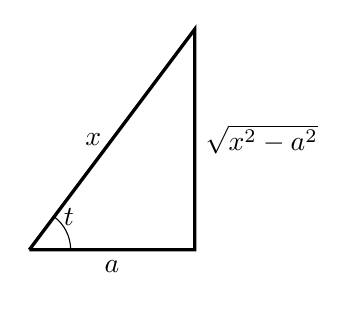
\begin{tikzpicture}[scale=.7]
\draw[very thick](0,0)--node[below]{$a$}(3,0)--node[right]{$\sqrt{x^2-a^2}$}(3,4)--node[left]{$x$}(0,0);
\draw(.75,0) arc (0:53.13:.75)node[right]{$t$};
\end{tikzpicture}
    \end{center}

    作正割代换.设$x=a\sec t\; \left(0<t<\frac{\pi}{2}\right)$,此函数在$t=\frac{\pi}{2}$点间断,在区间$\left[0,\frac{\pi}{2}\right)$上由$a$递增到$+\infty$,而在区间$\left(\frac{\pi}{2},\pi\right]$上由$-\infty$递增到$-a$.因此,$x=a\sec t$在$\left(0,\frac{\pi}{2}\right]$上的反函数是 
\[t=\arcsec\frac{x}{a}\quad \left(1<\frac{x}{a}<\infty,\; \text{即}x>a\right)\]
于是,当$x>a$时,有
\[\begin{split}
    \sqrt{x^2-a^2}&=\sqrt{a^2\sec^2 t-a^2}=\sqrt{a^2(\sec^2 t-1)}\\
    &=a\sqrt{\tan^2 t}=a|\tan t|\\
    &=a\tan t \quad \left(0\le t<\frac{\pi}{2}\right)
\end{split}\]
\[\dd x=\dd(a\sec t)=a\frac{\sin t}{\cos^2 t}\dd t\]
从而:
\[\begin{split}
    \Int \frac{1}{\sqrt{x^2-a^2}}\dd x&=\int\frac{1}{a\tan t}\cdot \frac{a\sin t}{\cos^2 t}\dd t\\
    &=\int \frac{1}{\cos t}\dd t=\ln|\sec t+\tan t|+C_1\\
    &=\ln\left|\frac{x}{a}+\frac{\sqrt{x^2-a^2}}{a}\right|+C_1\\
    &=\ln\left|x+\sqrt{x^2-a^2}\right|+C_1-\ln a=\ln\left|x+\sqrt{x^2-a^2}\right|+C
\end{split}\]
其中$C=C_1-\ln a$.

又函数$x=a\sec t$在$\left(\frac{\pi}{2},\pi\right]$上的反函数是
\[t=\arcsec\frac{x}{a}\quad \left(-\infty<\frac{x}{a}<-1,\; \text{即}x<-a\right)\]
于是,当$x<-a$时,有
\[\sqrt{x^2-a^2}=a\sqrt{\tan^2 t}=a|\tan t|=-a\tan t\quad \left(\frac{\pi}{2}<t\le \pi\right)\]
\[\dd x=\dd(a\sec t)=a\frac{\sin t}{\cos^2 t}\cdot \dd t\]
\[\begin{split}
    \Int \frac{1}{\sqrt{x^2-a^2}}\dd x&=\int-\frac{1}{a\tan t}\cdot \frac{a\sin t}{\cos^2 t}\dd t\\
    &=-\int \frac{1}{\cos t}\dd t=-\ln|\sec t+\tan t|+C_2\\
    &=-\ln\left|\frac{x}{a}-\frac{\sqrt{x^2-a^2}}{a}\right|+C_2\\
    &=-\ln\left|x-\sqrt{x^2-a^2}\right|+C_2+\ln a\\
    &=\ln\left|\frac{1}{x-\sqrt{x^2-a^2}}\right|+C'\qquad (C'=C+\ln a)\\
    &=\ln\left|\frac{x+\sqrt{x^2-a^2}}{a^2}\right|+C'=\ln\left|x+\sqrt{x^2-a^2}\right|+C'-\ln a^2\\
    &=\ln\left|x+\sqrt{x^2-a^2}\right|+C''\qquad (C''=C'-\ln a^2)
\end{split}\]
因此,不论$x>a$或$x<-a$,都有
\[\int\frac{\dd x}{\sqrt{x^2-a^2}}=\ln\left|x+\sqrt{x^2-a^2}\right|+C\]
\end{solution}

到现在为止,我们又得到四个重要的不定积分公式:

\begin{blk}{}
\begin{align}
\Int \frac{\dd x}{a^2+x^2}&=\frac{1}{a}\arctan\frac{x}{a}+C\\
\Int\frac{\dd x}{a^2-x^2}&=\frac{1}{2a}\ln\left|\frac{a+x}{a-x}\right|+C\\
 \Int\frac{\dd x}{\sqrt{a^2-x^2}}&=\arcsin\frac{x}{a}+C\\
\Int \frac{\dd x}{\sqrt{x^2\pm a^2}}&=\ln\left|x+\sqrt{x^2\pm a^2}\right|+C
\end{align}
\end{blk}

利用这些公式可以进一步求出许多不定积分.

\begin{blk}
 {类型A}
\[\int \frac{\dd x}{ax^2+bx+c}\]
\end{blk}

如果被积函数的分母可以分解因式,则把被积函数分解成部分分式,就很容易分项求出不定积分.

如分母不能分解因式,那么将它配方得
\[ax^2+bx+c=a\left(x+\frac{b}{2a}\right)^2+\frac{4ac-b^2}{4a}\]
于是
\begin{itemize}
    \item 当$4ac>b^2$时,上面不定积分归结到(4.10);
    \item 当$4ac<b^2$时,上面不定积分归结到(4.11).
\end{itemize}

\begin{example}
    求$\Int \frac{\dd x}{3x^2+x-1}$.
\end{example}

\begin{solution}
\[\begin{split}
    \Int \frac{\dd x}{3x^2+x-1}&=\frac{1}{3}\int \frac{\dd x}{\left(x+\frac{1}{6}\right)^2-\frac{13}{36}}\\
&=\frac{1}{3}\frac{1}{2\sqrt{\frac{13}{36}}}\ln\left|\frac{x+\frac{1}{6}-\frac{\sqrt{13}}{6}}{x+\frac{1}{6}+\frac{\sqrt{13}}{6}}\right|+C\\
&=\frac{1}{\sqrt{13}}\ln\left|\frac{6x+1-\sqrt{13}}{6x+1+\sqrt{13}}\right|+C
\end{split}\]    
\end{solution}

\begin{blk}
    {类型B}
   \[\int \frac{px+q}{ax^2+bx+c}\dd x\]
   \end{blk}

注意到$\frac{\dd}{\dd x}(ax^2+bx+c)=2ax+b$,被积函数的分子可以写成
\[px+q=\frac{p}{2a}(2ax+b)+q-\frac{pb}{2a}\]
于是
\[\int\frac{px+q}{ax^2+bx+c}\dd x=\frac{p}{2a}\int\frac{2ax+b}{ax^2+bx+c}\dd x+\left(q-\frac{bp}{2a}\right)\int\frac{\dd x}{ax^2+bx+c}\]
等式右端第一项是$\frac{p}{2a}\ln(ax^2+bx+c)$,第二项可归结到类型A.

\begin{example}
    求$\Int \frac{5x-1}{3x^2+x+2}\dd x$.
\end{example}

\begin{solution}
\[\begin{split}
    \Int \frac{5x-1}{3x^2+x+2}\dd x&=\frac{5}{6}\int \frac{6x+1}{3x^2+x+2}\dd x-\frac{11}{6}\int\frac{\dd x}{3x^2+x+2}\\
&=\frac{5}{6}\ln(3x^2+x+2)-\frac{11}{6}\cdot \frac{1}{3}\cdot \int \frac{\dd x}{\left(x+\frac{1}{6}\right)^2+\frac{23}{36}}\\
&=\frac{5}{6}\ln(3x^2+x+2)-\frac{11}{6}\cdot\frac{1}{3}\cdot\frac{6}{\sqrt{23}}\arctan\frac{6x+1}{\sqrt{23}}+C\\
&=\frac{5}{6}\ln(3x^2+x+2)-\frac{11}{3\sqrt{23}}\arctan\frac{6x+1}{\sqrt{23}}+C
\end{split}\]    
\end{solution}

\begin{blk}{类型C}
\[\int \frac{\dd x}{\sqrt{ax^2+bx+c}}\]
\end{blk}

\begin{itemize}
    \item 若$a>0$, 则被积函数的根底式经配方后,所求积分可归结到积分公式(4.13);
    \item  若$a<0$, 则此积分可归结到积分公式(4.12).
\end{itemize}

\begin{example}
    求$\Int \frac{\dd x}{\sqrt{2+x-3x^2}}$
\end{example}

\begin{solution}
    \[\begin{split}
        \Int \frac{\dd x}{\sqrt{2+x-3x^2}}&=\frac{1}{\sqrt{3}}\int \frac{\dd x}{\sqrt{\frac{2}{3}+\frac{1}{3}x-x^2}}\\
        &=\frac{1}{\sqrt{3}}\int \frac{\dd x}{\sqrt{\frac{25}{36}-\left(x-\frac{1}{6}\right)^2}}\\
        &=\frac{1}{\sqrt{3}}\arcsin\frac{x-\frac{1}{6}}{\frac{5}{6}}+C\\
        &=\frac{1}{\sqrt{3}}\arcsin\frac{6x-1}{5}+C       
    \end{split}\]
\end{solution}

\begin{blk}{类型D}
\[\int \frac{px+q}{\sqrt{ax^2+bx+c}}\dd x\]
\end{blk}

被积函数的分子可写成
\[px+q=\frac{p}{2a}(2ax+b)+q-\frac{pb}{2a}\]
所以
\[
    \int \frac{px+q}{\sqrt{ax^2+bx+c}}\dd x=\frac{p}{2a}\int \frac{2ax+b}{\sqrt{ax^2+bx+c}}\dd x+\left(q-\frac{pb}{2a}\right)\int\frac{\dd x}{\sqrt{ax^2+bx+c}}
\]
等式右端第一个积分等于被积函数的分母的2倍,即$2\sqrt{ax^2+bx+c}$, 第二个是类型C的积分.

\begin{example}
    求$\Int \frac{5x-1}{\sqrt{3x^2+x+2}}\dd x$.
\end{example}

\begin{solution}
    \[\begin{split}
        \Int \frac{5x-1}{\sqrt{3x^2+x+2}}\dd x&=\frac{5}{6}\int \frac{6x+1}{\sqrt{3x^2+x+2}}\dd x-\frac{11}{6}\int \frac{\dd x}{\sqrt{3x^2+x+2}}\\
&=\frac{5}{6}\cdot 2\sqrt{3x^2+x+2}\\
&\qquad -\frac{11}{6}\cdot\frac{1}{\sqrt{3}}\ln\left[x+\frac{1}{6}+\sqrt{\left(x+\frac{1}{6}\right)^2+\frac{23}{36}}\right]+C\\
&=\frac{5}{3}\sqrt{3x^2+x+2}-\frac{11}{6\sqrt{3}}\ln\left[x+\frac{1}{6}+\sqrt{\left(x+\frac{1}{6}\right)^2+\frac{23}{36}}\right]+C        
    \end{split}\]
\end{solution}

\begin{blk}{类型E}
    \[\int \frac{\dd x}{x\sqrt{ax^2+bx+c}}\]
\end{blk}

作变量代换$x=\frac{1}{y}$,所求积分可化为类型C.因为$\dd x=-\frac{1}{y^2}\dd y$,并且
\[\int \frac{\dd x}{x\sqrt{ax^2+bx+c}}=\int\frac{-\frac{1}{y^2}\dd y}{\frac{1}{y}\sqrt{\frac{a}{y^2}+\frac{b}{y}+c}}=-\int\frac{\dd y}{\sqrt{a+by+cy^2}}\]

\begin{example}
    求$\Int\frac{\dd x}{x\sqrt{x^2+x+1}}$
\end{example}

\begin{solution}
\[\begin{split}
    \Int\frac{\dd x}{x\sqrt{x^2+x+1}}&=-\int \frac{-\frac{1}{y^2}\dd y}{\frac{1}{y}\sqrt{\frac{1}{y^2}+\frac{1}{y}+1}}=-\int \frac{\dd y}{\sqrt{y^2+y+1}}\\
    &=-\int \frac{\dd y }{\sqrt{\left(y+\frac{1}{2}\right)^2+\frac{3}{4}}}  \\
    &=-\ln \left[y+\frac{1}{2}+\sqrt{\left(y+\frac{1}{2}\right)^2+\frac{3}{4}}\right]+C \\
    &=-\ln \left[y+\frac{1}{2}+\sqrt{y^2+y+1}\right]+C\\
    &=-\ln\left[\frac{1}{x}+\frac{1}{2}+\sqrt{\frac{1}{x^2}+\frac{1}{x}+1}\right]+C\\
    &=-\ln\frac{2+x+2\sqrt{x^2+x+1}}{2x}+C
\end{split}\]
\end{solution}
    
\begin{ex}
\begin{enumerate}
    \item 求下列不定积分:
\begin{multicols}{2}
\begin{enumerate}
    \item $\Int \frac{1}{1+\sqrt[3]{x}}\dd x$
    \item $\Int \frac{1}{(x+2) \sqrt{x+1}}\dd x$
    \item $\Int  \frac{x}{\sqrt[3]{1-x}}\dd x $
    \item $\Int \frac{\sqrt{x}}{\sqrt[3]{x^{2}}-\sqrt[4] {x}}\dd x$
    \item $\Int  \frac{\sqrt{x^{2}-a^{2}}}{x}\dd x $
    \item $\Int  \frac{\sqrt{x^{2}-a^{2}}}{x^{2}}\dd x$
    \item $\Int  \frac{\sqrt{a^{2}-x^{2}}}{x}\dd x$
    \item $\Int \frac{\sqrt{a^{2}-x^{2}}}{x^{2}}\dd x$
    \item $\Int \frac{x^{2}}{\sqrt{1-x^{2}}}\dd x$
    \item $\Int \frac{1}{x^{4} \sqrt{1+x^{2}}}\dd x$
\end{enumerate}
\end{multicols}

    \item 求下列不定积分:
\begin{multicols}{2}
\begin{enumerate}
\item $\Int \frac{1}{\sqrt{4 x^{2}+6 x}}\dd x $
\item $\Int \frac{x}{\sqrt{4 x^{2}+6 x}}\dd x$
\item $\Int  \frac{1}{\sqrt{1-x-4 x^{2}}}\dd x$
\item $\Int \frac{x+1}{\sqrt{1-x-4 x^{2}}}\dd x$
\item $\Int \frac{1}{x \sqrt{x^{2}+1}}\dd x$
\item $\Int \frac{1}{x \sqrt{1-x^{2}}}\dd x$
\item $\Int \frac{1}{x \sqrt{x^{2}-4 x}}\dd x$
\item $\Int \sqrt{\frac{x-1}{x+1}}\dd x$  
\end{enumerate}
\end{multicols}

\end{enumerate}    
\end{ex}

\subsection{有理函数的积分}
如果$P(x)$, $Q(x)$是两个多项式,则$\Int \frac{P(x)}{Q(x)}\dd x$可以化
归为下列类型的积分:
\begin{center}
\begin{tabular}{p{.3\textwidth}p{.3\textwidth}}
        $\Int \frac{A \dd x}{x-a}$ & $\Int \frac{A \dd x}{(x-a)^{n}}$ \\
        $\Int \frac{p x+q}{x^{2}+b x+c} \dd x$ & $\Int \frac{p x+q}{\left(x^{2}+b x+c\right)^{n}} \dd x$
\end{tabular}
\end{center}

对这些积分,我们是有办法的.下面我们通过举例来说明求这些积分的大概的方法.

如果有理分式的分子次数高于分母的次数时,则只要作一次除法就可以把它写成一个多项式与一个真分式的和,而前者是容易求积的.所以我们只须注意真分式的积分如何求.

\begin{example}
    求$\Int \frac{x^3+x+1}{x^2+1}\dd x$
\end{example}

\begin{solution}
    \[\begin{split}
        \Int \frac{x^3+x+1}{x^2+1}\dd x&=\int\left(x+\frac{1}{x^2+1}\right)\dd x\\
&=\int x\dd x+\int\frac{\dd x}{1+x^2}\\
&=\frac{x^2}{2}+\arctan x+C        
    \end{split}\]
\end{solution}

\begin{example}
    求$\Int \frac{\dd x}{x^4-1}$
\end{example}

\begin{solution}
$\because\quad x^4-1=(x-1)(x+1)(x^2+1)$

$\therefore\quad \frac{1}{x^4-1}=\frac{A}{x-1}+\frac{B}{x+1}+\frac{Cx+D}{x^2+1}$

把等式右端通分,再比较两端系数,于是等式
\[A (x^2+1) (x+1)+B(x^2+1)(x-1)+(Cx+D) (x^2-1)=1\]
的左边多项式的$x^3,x^2,x$的系数应为零,常数项应为1, 从而得到
\begin{numcases}{}
    A+B+C=0\\
    A-B+D=0\\
    A+B-C=0\\
    A-B-D=1
\end{numcases}
由$(4.14)+(4.16)$和$(4.15)+(4.17)$得到:
\[A+B=0,\qquad A-B=\frac{1}{2}\]
解得:
\[A=\frac{1}{4},\quad B=-\frac{1}{4},\quad C=0,\quad D=-\frac{1}{2}\]
即:
\[\frac{1}{x^4-1}=\frac{1}{4(x-1)}-\frac{1}{4(x+1)}-\frac{1}{2(x^2+1)}\]
从而
\[\begin{split}
    \int\frac{\dd x}{x^4-1}&=\frac{1}{4}\int \frac{\dd x}{x-1}-\frac{1}{4}\int\frac{\dd x}{x+1}-\frac{1}{2}\int\frac{\dd x}{1+x^2}\\
    &=\frac{1}{4}\ln\left|\frac{x-1}{x+1}\right|-\frac{1}{2}\arctan x+C
\end{split}\]
\end{solution}

\begin{example}
求$\Int \frac{3x^2+x-2}{(x-2)^2(1-2x)}\dd x$
\end{example}

\begin{solution}
设$\frac{3x^2+x-2}{(x-2)^2(1-2x)}=\frac{A}{1-2x}+\frac{B}{x-2}+\frac{C}{(x-2)^2}$,则
\[3x^2+x-2=A(x-2)^2+B(1-2x)(x-2)+C(1-2x)\]

令$1-2x=0$,则$A=-\frac{1}{3}$;令$x-2=0$,则$C=-4$. 比较等式两端$x^2$的系数,得
\[3=A-2B\quad\Rightarrow\quad B=-\frac{5}{3}\]
所以
\[\frac{3x^2+x-2}{(x-2)^2(1-2x)}=-\frac{1}{3(1-2x)}-\frac{5}{3(x-2)}-\frac{4}{(x-2)^2}\]
从而
\[\begin{split}
\int \frac{3x^2+x-2}{(x-2)^2(1-2x)}\dd x &=\frac{1}{6}\int \frac{\dd x}{x-\frac{1}{2}}-\frac{5}{3}\int \frac{\dd x}{x-2}-4\int \frac{\dd x}{(x-2)^2}\\
&=\frac{1}{6}\ln\left|x-\frac{1}{2}\right|-\frac{5}{3}\ln|x-2|+\frac{4}{x-2}+C
\end{split}\]
\end{solution}

三角函数有理式的积分
\[\int R (\sin x,\cos x) \dd x\]
恒可用“半角变换”法,即设$t=\tan\frac{x}{2}$或$x=2\arctan t$化为$t$的有理函数的积分.

事实上,由$t=\tan\frac{x}{2}$, 知
\[\begin{split}
\sin x&=\frac{2 \sin \frac{x}{2} \cos \frac{x}{2}}{\sin ^{2} \frac{x}{2}+\cos ^{2} \frac{x}{2}}=\frac{2 \tan \frac{x}{2}}{1+\tan^{2} \frac{x}{2}}=\frac{2 t}{1+t^{2}}\\
\cos x &=\frac{\cos ^{2}-\frac{x}{2}-\sin ^{2} \frac{x}{2}}{\sin ^{2} \frac{x}{2}+\cos ^{2} \frac{x}{2}}=\frac{1-\tan^{2} \frac{x}{2}}{1+\tan^{2} \frac{x}{2}} 
=\frac{1-t^{2}}{1+t^{2}}
\end{split}\]
又由 $x=2 \arctan t$, 知
\[\dd x=\frac{2 \dd t}{1+t^{2}}\]
于是
\[
\int R(\sin x,  \cos x) \dd x=\int R\left(\frac{2 t}{1+t^{2}}, \frac{1-t^{2}}{1+t^{2}}\right) \cdot \frac{2}{1+t^{2}} \dd x 
\]
上式右端是 $t$ 的有理函数.

\begin{example}
    求$\Int \frac{\dd\theta}{\sin\theta}$.
\end{example}

\begin{solution}
令$t=\tan\frac{\theta}{2}$,则:$\theta=2\arctan t,\quad \dd\theta=\frac{2\dd t}{1+t^2}$,从而:
\[\begin{split}
    \int\frac{\dd\theta}{\sin\theta}=\int\frac{1+t^2}{2t}\cdot \frac{2\dd t}{1+t^2}&=\int\frac{\dd t}{t}\\
    &=\ln|t|+C=\ln\left|\tan\frac{\theta}{2}\right|+C
\end{split}\]
又$\tan\frac{\theta}{2}=\frac{\sin\frac{\theta}{2}}{\cos\frac{\theta}{2}}=\frac{2\sin^2 \frac{\theta}{2}}{2\sin\frac{\theta}{2}\cos \frac{\theta}{2}}=\frac{1-\cos\theta}{\sin\theta}=\csc\theta-\cot\theta$,
所以
\[\int\frac{\dd\theta}{\sin\theta}=\ln\left|\tan\frac{\theta}{2}\right|+C=\ln|\csc\theta-\cot\theta|+C\]    
\end{solution}

\begin{example}
    求$\Int \frac{\dd\theta}{3+2\cos\theta}$
\end{example}

\begin{solution}
    令$t=\tan\frac{\theta}{2}$,则:$\dd\theta=\frac{2\dd t}{1+t^2}$,于是
\[\begin{split}
    \Int \frac{\dd\theta}{3+2\cos\theta}=\int\frac{\frac{2\dd t}{1+t^2}}{3+2\frac{1-t^2}{1+t^2}}&=\int \frac{2\dd t}{5+t^2}\\
    &=\frac{2}{\sqrt{5}} \arctan\frac{t}{\sqrt{5}}+C\\
    &=\frac{2}{\sqrt{5}}\arctan\left(\frac{1}{\sqrt{5}}\tan\frac{\theta}{2}\right)+C
\end{split}\]
\end{solution}

\begin{ex}
\begin{enumerate}
\item 求下列不定积分:
\begin{multicols}{2}
\begin{enumerate}
\item  $\Int \frac{1}{x^{2}-3 x+2}\dd x$
\item  $\Int  \frac{x}{x^{2}-3 x+2}\dd x$
\item  $\Int  \frac{x^{2}}{x^{2}-3 x+2}\dd x$
\item  $\Int \frac{x^{2}+1}{x+3}\dd x$
\item  $\Int \frac{1}{x^{2}-3 x+1}\dd x$
\item  $\Int \frac{x}{x^{2}-3 x+1}\dd x$
\item  $\Int \frac{x^{2}}{x^{2}-3 x+1}\dd x$
\end{enumerate}
\end{multicols}

\item 求下列不定积分:
\begin{multicols}{2}
    \begin{enumerate}
        \item  $\Int  \frac{\cos \theta \dd \theta}{1+\sin ^{2} \theta}$
        \item  $\Int \frac{\sin x+\cos x}{\cos ^{2} x}\dd x$
        \item  $\Int  \frac{\dd x}{4 \cos x+3 \sin x+5}$
        \item  $\Int \frac{\sin x}{\cos x+\sin x}\dd x$
    \end{enumerate}
\end{multicols}
\end{enumerate}
\end{ex}

\subsection{分部积分法}

分部积分法是从两个函数乘积的微分公式得到的求积分方法.

设$u=u(x)$, $v=v(x)$是两个可微函数,乘积$u\cdot v$的微分法则是$$\dd (u\cdot v) =u\dd v+v\dd u$$
移项,得$u\dd v=\dd (w\cdot v) -v\dd u$,
两边积分得
\begin{equation}
    \int u\dd v=u\cdot v-\int v\dd u
\end{equation}
公式(4.18)表示如果积分$\Int u\dd v=\Int u(x)v'(x)\dd x$不可能直接求出,就改为求积分$\Int v\dd u=\Int v(x)u'(x)\dd x$, 设$F(x)$是$v(x)\cdot u'(x)$的一个原函数,那么$u(x)\cdot v(x)-F(x)$是$u(x)v'(x)$的一个原函数,用公式(4.18)求不定积分的方法叫做\textbf{分部积分法},公式(4.18)叫做\textbf{分部积分公式}.

\begin{example}
    求$\Int x\sin 3x\dd x$.
\end{example}

\begin{solution}
被积函数$x\sin3x$不能由前面的基本积分表求出它的原函数,我们把$x\sin3x$分成两部分,设$u(x)=x$, $v'(x)=\sin3x$, 于是
\[\int v' (x) \dd x= \int \sin3x\dd x=-\frac{\cos3x}{3}+C\]
即$v(x)=-\frac{\cos3x}{3}$是$v'(x)=\sin3x$的一个原函数,根据公
式(4.18),有
\[\begin{split}
    \int x\sin 3x\dd x&=\int x\dd\left(-\frac{\cos 3x}{3}\right)\\
    &=x\left(-\frac{\cos 3x}{3}\right)-\int\left(-\frac{\cos3x}{3}\right)\dd x \\
&=-\frac{x\cos 3x}{3}+\frac{1}{3}\int \cos 3x\dd x\\
&=-\frac{x\cos 3x}{3}+\frac{\sin 3x}{9}+C
\end{split}\]
\end{solution}

运用公式(4.18)时,应首先将被积表达式分成函数$u(x)$和微分$\dd v=v'(x)\dd x$两部分,选取$u(x)$和$v'(x)\dd x$的原则是:
\begin{itemize}
    \item 充当微分部分的$v'(x)\dd x$, 其$v'(x)$的原函数能够比较容易地求出;
\item 
充当$u(x)$的部分经求微商后要化简,以便使积分$\Int v\dd u$较$\Int u\dd v$简单,容易求出结果.
\end{itemize}

在应用分部积分法求不定积分时,往往要连续使用这个
方法多次才能求出最后结果.

我们把能够应用分部积分法求积分的例题分为以下几类:

\begin{blk}
 {类型A} 被积函数是$x^ne^{ax}$, $x^n\sin ax$, $x^n\cos ax$, 其中$x$的方幂因子经求微商后降次,而非$x$的方幂因子的原函数是容易求得的.   
\end{blk}

\begin{example}
求$\Int x^2 e^{2x}\dd x$.
\end{example}

\begin{solution}
\[\begin{split}
    \Int x^2 e^{2x}\dd x=\int x^2 \dd\left(\frac{e^{2x}}{2}\right)&=\frac{x^2e^{2x}}{2}-\int \frac{e^{2x}}{2}\dd(x^2)\\
&=\frac{x^2e^{2x}}{2}-\int xe^{2x}\dd x=\frac{x^2e^{2x}}{2}-\left(\frac{xe^{2x}}{2}-\int \frac{e^{2x}}{2}\dd x\right)\\
&=\frac{x^2}{2}e^{2x}-\frac{x}{2}e^{2x}+\frac{e^{2x}}{4}+C\\    
&=e^{2x}\left(\frac{x^2}{2}-\frac{x}{2}+\frac{1}{4}\right)+C
\end{split}\]
\end{solution}

\begin{blk}
    {类型B} 被积函数是$x^n\sin^{-1}x$, $x^n\tan^{-1}x$, $x^n\ln x$, 其中乘积中的因子$\tan^{-1} x$, $\ln x$的导数是$x$的有理函数,$\sin^{-1}x$的
导数是$\frac{1}{\sqrt{1-x^2}}$,
它们的积分可求,而$x^n$的原函数是$\frac{x^{n+1}}{n+1}$.
\end{blk}


\begin{example}
求$\Int x\arctan x\dd x$.    
\end{example}

\begin{solution}
  \[\begin{split}
    \Int x\arctan x\dd x=\int \arctan x \dd\left(\frac{x^2}{2}\right)&=\frac{x^2\arctan x}{2}-\int \frac{x^2}{2}\dd(\arctan x)\\
    &=\frac{x^2\arctan x}{2}-\frac{1}{2}\int \frac{x^2}{1+x^2}\dd x\\
    &=\frac{x^2\arctan x}{2}-\frac{1}{2}\int \left(1-\frac{1}{1+x^2}\right)\dd x\\
    &=\frac{x^2\arctan x}{2}-\frac{1}{2}x+\frac{1}{2}\arctan x+C
  \end{split}\]  
\end{solution}


\begin{example}
    求$\Int x^3\ln x\dd x$.
\end{example}

\begin{solution}
\[\begin{split}
    \Int x^3\ln x\dd x=\int \ln x\dd\left(\frac{x^4}{4}\right)&=\frac{x^4}{4}\ln x-\int \frac{x^4}{4}\dd(\ln x)\\
    &= \frac{x^4}{4}\ln x-\int  \frac{x^4}{4}\cdot \frac{1}{x}\dd x\\
    &= \frac{x^4}{4}\ln x- \frac{x^4}{16}+C
\end{split}\]
\end{solution}

\begin{blk}
    {类型C} 被积函数是$\sin^{-1}x$, $\tan^{-1}x$, $\ln x$, 这里没有乘积的形式,不妨设$v'(x)=1$.
\end{blk}

\begin{example}
求$\Int \arcsin x\dd x$.
\end{example}

\begin{solution}
\[\begin{split}
    \Int \arcsin x\dd x=x\arcsin x-\int x\dd(\arcsin x)&=x\arcsin x-\int\frac{x}{\sqrt{1-x^2}}\dd x  \\
    &=x\arcsin x+\frac{1}{2}\int \frac{\dd(1-x^2)}{\sqrt{1-x^2}}\\
    &=x\arcsin x+\frac{1}{2}\cdot 2\sqrt{1-x^2}+C\\
    &=x\arcsin x+\sqrt{1-x^2}+C
\end{split}\]

另解:设$y=\arcsin x,\; -1\le x\le 1$,则$\sin y=x,\; -\frac{\pi}{2}\le y\le \frac{\pi}{2}$
\[\begin{split}
    \Int \arcsin x\dd x=x\arcsin x-\int x\dd(\arcsin x)&=y\sin y-\int \sin y \dd y\\
    &=y\sin y+\cos y+C\\
    &=x\arcsin x+\sqrt{1-\sin^2 y}+C\\
    &=x\arcsin x+\sqrt{1-x^2}+C
\end{split}\]
\end{solution}

\begin{example}
    求$\Int \ln^2 x\dd x$.
\end{example}

\begin{solution}
    \[\begin{split}
        \Int \ln^2 x\dd x=x(\ln x)^2-\int x\dd (\ln^2 x)&=x(\ln x)^2-\int x\cdot 2\ln x\cdot \frac{1}{x}\dd x\\
        &=x(\ln x)^2-2\int \ln x\dd x\\
        &=x(\ln x)^2-2\left[x\ln x-\int x\d(\ln x)\right]\\
        &=x(\ln x)^2-2x\ln x+2\int \dd x\\
        &=x(\ln x)^2-2x\ln x+2x+C   
    \end{split}\]
\end{solution}

\begin{blk}
    {类型D} 被积函数是$e^{ax}\sin bx$, $\sec^3 x$, $\sqrt{a^2+x^2}$. 对于这类例题,两次使用这个方法可以得到含有这个积分作未知元的一次方程.
\end{blk}

\begin{example}
    求$\Int e^{ax}\sin bx\dd x$
\end{example}

\begin{solution}
\[\begin{split}
    I=\Int e^{ax}\sin bx\dd x
    &=\int \sin bx \dd\left(\frac{e^{ax}}{a}\right)\\
&=\sin bx\cdot \frac{e^{ax}}{a}-\int \frac{e^{ax}}{a}\dd(\sin bx)\\
&=\sin bx\cdot \frac{e^{ax}}{a}-\int \frac{e^{ax}}{a}b\cos bx\dd x\\
&=\sin bx\cdot \frac{e^{ax}}{a}-\frac{b}{a}\int \cos bx\dd\left(\frac{e^{ax}}{a}\right)\\
&=\sin bx\cdot \frac{e^{ax}}{a}-\frac{b}{a}\left[\cos bx\cdot \frac{e^{ax}}{a}-\int \frac{e^{ax}}{a}\dd\left(\cos bx\right)\right]\\
&=\sin bx\cdot \frac{e^{ax}}{a}-\frac{b}{a^2}\cos bx\cdot e^{ax}-\frac{b^2}{a^2}\int e^{ax}\sin bx\dd x\\
&=\sin bx\cdot \frac{e^{ax}}{a}-\frac{b}{a^2}\cos bx\cdot e^{ax}-\frac{b^2}{a^2}I
\end{split}\]
所以:
\[\begin{split}
    I\left(1+\frac{b^2}{a^2}\right)&=\frac{1}{a}\sin bx\cdot e^{ax}-\frac{b}{a^2}\cos bx\cdot e^{ax}\\
    I&=\frac{e^{ax}(a\sin bx-b\cos bx)}{a^2+b^2}+C
\end{split}\]    
\end{solution}

\begin{example}
    求$\Int \sqrt{a^2+x^2}\dd x$.
\end{example}

\begin{solution}
\[    \begin{split}
    I =\int \sqrt{a^{2}+x^{2}} \dd x 
    &=x \sqrt{a^{2}+x^{2}}-\int x \dd\left(\sqrt{a^{2}+x^{2}}\right) \\
    &=x \sqrt{a^{2}+x^{2}}-\int \frac{x^{2}}{\sqrt{a^{2}+x^{2}}} \dd x \\
    &=x \sqrt{a^{2}+x^{2}}-\int \frac{x^{2}+a^{2}}{\sqrt{a^{2}+x^{2}}} \dd x+\int \frac{a^{2}}{\sqrt{a^{2}+x^{2}}} \dd x \\
    &=x \sqrt{a^{2}+x^{2}}-I+a^{2} \ln \left(x+\sqrt{a^{2}+x^{2}}\right)
    \end{split}\]
    所以
\[    I=\frac{1}{2} x \sqrt{a^{2}+x^{2}}+\frac{1}{2} a^{2} \ln \left(x+\sqrt{a^{2}+x^{2}}\right)\]
\end{solution}

应用分部积分公式(4.18)还能导出一些求积分的递归公式.所谓求积分的递归公式就是建立一个被积函数含有正整数$n$的积分与被积函数含有非负整数$n-1$或$n-2$的积分的关系式.每次要求$n=k$时的积分,重复利用这个关系式总能回到当$n=0, 1, 2$时的起始积分,于是所求积分总能用$n$的起始值$n=0, 1, 2$中的一个已知积分表示出来.这也就是递归的
意思.
    
\begin{example}
    求$\Int \sin^n x\dd x$.
\end{example}

\begin{solution}
当$n=0$时,$I_0=\Int (\sin x)^0\dd x=\Int \dd x=x+C$

又:
\[
\begin{split}
I_{n} =\int \sin ^{n} x \dd x&=\int \sin ^{n-1} x \dd(-\cos x) \\
&=-\cos x \sin ^{n-1} x+\int \cos x \dd\left(\sin ^{n-1} x\right) \\
&=-\cos x \sin ^{n-1} x+(n-1) \int \cos x \sin ^{n-2} x \cdot \cos x \dd x \\
&=-\cos x \sin ^{n-1} x+(n-1) \int \sin ^{n-2} x\left(1-\sin ^{2} x\right) \dd x
\end{split}
\]
所以
$$
I_{n}=-\cos x \sin ^{n-1} x+(n-1) I_{n-2}-(n-1) I_{n}
$$
即
\begin{equation}
   n I_{n}=-\cos x \sin ^{n-1} x+(n-1) I_{n-2} 
\end{equation}

现在我们用递归关系(4.19)来求 $\Int \sin ^{4} x \dd x$. 
设 $I_{4}=\Int \sin ^{4} x \dd x$, 于是
\begin{align}
4 I_{4}&=-\cos x \sin ^{3} x+3 I_{2} \\
2 I_{2}&=-\cos x \sin x+I_{0} 
\end{align}
将(4.21)代入(4.20)得:
\[\begin{split}
    4I_4&=-\cos x\sin^3 x+3\left(-\frac{\sin x\cos x}{2}+\frac{1}{2}I_0\right)\\
    &=-\cos x\sin^3 x-\frac{3}{2}\cos x\sin x+\frac{3}{2}x+C
\end{split}\]
所以
\[I_4=\int \sin^4 x\dd x=-\frac{1}{4}\cos x\sin^3 x-\frac{3}{8}\cos x\sin x+\frac{3}{8}x+C\]


\begin{ex}
\begin{enumerate}
    \item 求下列不定积分:
\begin{multicols}{2}
\begin{enumerate}
    \item $\Int x \sin x\dd x$
    \item $\Int x \cos 3 x\dd x$
    \item $\Int x \sin ^{2} \frac{x}{2}\dd x$
    \item $\Int x e^{-x}\dd x$
    \item $\Int (x-1) e^{x}\dd x$
    \item $\Int \left(x^{2}+x\right) e^{-x}\dd x$
    \item $\Int  x \sec ^{2} x\dd x$
    \item $\Int  x \arcsin x\dd x$
    \item $\Int  \frac{\arcsin x}{x^{2}}\dd x$
    \item $\Int  \frac{\arctan x}{x^{2}}\dd x$
    \item $\Int  x^{2} e^{3 x}\dd x$
    \item $\Int  e^{a x} \sin ^{2} b x\dd x$
    \item $\Int  \sin x \cdot \ln (\tan x)\dd x$
    \item $\Int  x^{2} \arctan x\dd x$
    \item $\Int  \frac{x^{2} e^{x}\dd x}{(x+2)^{2}}$
    \item $\Int \frac{x e^{x}}{(x+1)^{2}}\dd x$
\end{enumerate}
\end{multicols}
 \item   求下列不定积分:    
   \begin{multicols}{2}
        \begin{enumerate}
    \item $\Int \arctan \sqrt{x}\dd x$
    \item $\Int \ln ^{2} x \dd {x}$
    \item $\Int \ln \left(x+\sqrt{1+x^{2}}\right)\dd x$
    \item $\Int (\arcsin x)^{2}\dd x$
    \item $\Int \sin(\ln x)\dd x$
    \item $\Int \sqrt{4+x^2}\dd x$
\end{enumerate}
\end{multicols}
\end{enumerate}
\end{ex}
\end{solution}
    
\section{定积分的计算与应用}

\subsection{定积分的计算}

由微积分的基本定理得知,定积分$\Int^b_a f(x)\dd x$的计算归结为不定积分$\Int f(x)\dd x$的计算,由后者计算得到$f(x)$的原函数$F(x)$, 则
\[\Int^b_a f(x)\dd x=F (x)\Bigg|^b_a=F (b) -F (a)\] 
于是计算不定积分的各种方法也可移植过来求定积分.

\subsubsection{定积分的换元积分法}

第一换元法:设$\Int f(u)\dd u=F(u)$, $u=\varphi(x)$可微,
那么
\[\begin{split}
    \int^b_a f(\varphi(x))\varphi'(x)\dd x&=\int^{\varphi(b)}_{\varphi(a)}f(u)\dd u\\
    &=F(u)\Big|^{\varphi(b)}_{\varphi(a)}=F[{\varphi(b)}]-F[{\varphi(a)}]
\end{split}\]

\begin{example}
    求$\Int^{\tfrac{\pi}{2}}_0 \sin^3x \cos x\dd x$.
\end{example}

\begin{solution}
    因为
\[\int \sin^3x\cos x\dd x= \int \sin^3x\dd (\sin x) =\frac{1}{4}\sin^4x+C\]
所以
\[\begin{split}
    \Int^{\tfrac{\pi}{2}}_0 \sin^3x \cos x\dd x&=\frac{1}{4}\sin^4 x\Big|^{\tfrac{\pi}{2}}_0 \\
    &=\frac{1}{4}\left[\sin^4\frac{\pi}{4}-0\right]=\frac{1}{4}
\end{split}\]
\end{solution}

\begin{blk}
 {定理1(第二种变量代换法)}设$f(x)$在$[a,b]$上连续,作代换$x=\varphi (t)$, 其中$\varphi (t)$在某一闭区间$[\alpha,\beta]$上有连续导数$\varphi '(t)$, 当$\alpha\le t\le \beta$时,$a\le \varphi (t)\le b$, 且$\varphi (\alpha)=a$, $\varphi (\beta)=b$, 那么
\[\int^b_a f(x) \dd x= \int^{\beta}_{\alpha} f [\varphi  (t) ] \varphi ' (t) \dd t\]   
\end{blk}

\begin{proof}
    设$f(x)$的一个原函数是$G(x)$, 即有
\[\frac{\dd}{\dd x}G (x) =f (x)\]
于是由微积分基本定理得
\begin{equation}
    \int^b_a f (x)\dd x=G(x)\Big|^b_a=G(b) -G (a)
\end{equation}
根据复合函数求导法则,知
\[\begin{split}
    \frac{\dd}{ \dd t}G[\varphi  (t) ] &=\frac{\dd}{ \dd x}G (x)\cdot  \frac{\dd}{ \dd t}\varphi  (t)\\
    &=f(x)\cdot \varphi'(t)=f[\varphi(t)]\varphi'(t)
\end{split}\]
所以$G[\varphi (t)]$是$f[\varphi (t)]\varphi '(t)$的一个原函数,从而
\begin{equation}
    \begin{split}
\int^{\beta}_{\alpha} f [\varphi  (t) ] \varphi ' (t) \dd t&=G [\varphi  (t) ]\Big|^{\beta}_{\alpha}\\
&=       G [\varphi  (\beta) ] -G [\varphi  (\alpha) ]=G (b) -G (a)
    \end{split}
\end{equation}
因为(4.22)(4.23)两个积分相等,所以
\[\int^b_a f(x) \dd x= \int^{\beta}_{\alpha} f [\varphi  (t) ] \varphi ' (t) \dd t\]
\end{proof}

这个公式与不定积分的换元公式很类似,所不同的是,后者最后需要将变量还原,而现在只须把积分限作相应的改变.

\begin{example}
    求$\Int^a_0 \sqrt{a^2-x^2}\dd x$
\end{example}

\begin{solution}
作代换$x=a\sin t$,当$x$从0变到$a$时,相应地$t$自0变到$\frac{\pi}{2}$,于是
\[\begin{split}
    \Int^a_0 \sqrt{a^2-x^2}\dd x=a^2\int^{\tfrac{\pi}{2}}_0 \cos ^2 t\dd t&=a^2\int^{\tfrac{\pi}{2}}_0 \frac{1+\cos 2t}{2}\dd t\\
    &=\frac{a^2}{2}\left(t+\frac{1}{2}\sin 2t\right)\Bigg|^{\tfrac{\pi}{2}}_0=\frac{\pi a^2}{4} 
\end{split}\]
\end{solution}

\begin{example}
    求$\Int^4_0 \frac{1}{1+\sqrt{x}}\dd x$
\end{example}

\begin{solution}
    设$x=u^2$,于是
\[\frac{1}{1+\sqrt{x}}=\frac{1}{1+u},\qquad \dd x=2u\dd u\]
定限:当$x=0$时,从变换$\sqrt{x}=u$中解出$u=0$;当$x=4$时,解出$u=2$. 于是
\[\begin{split}
    \Int^4_0 \frac{1}{1+\sqrt{x}}\dd x=\int^2_0 \frac{1}{1+u}\cdot 2u\dd u&=2\int^2_0 \left(1-\frac{1}{1+u}\right)\dd u\\
    &=2\left[u-\ln(1+u)\right]\Big|^2_0=2(2-\ln 3)
\end{split}\]
\end{solution}

\begin{example}
求证:$\Int^a_0 f(x)\dd x=\Int^a_0 f(a-x)\dd x$
\end{example}

\begin{proof}
    设$x=a-t$,则$\dd x=-\dd t$,且当$x=0$时,$t=a$;当$x=a$时,$t=0$. 于是:
\[\begin{split}
    \Int^a_0 f(x)\dd x=\int^0_a f(a-t)(-\dd t)&=-\int^0_a f(a-t)\dd t\\
    &=\int^a_0 f(a-t)\dd t=\Int^a_0 f(x)\dd x
\end{split}\]
\end{proof}

我们在第三节曾指出,使用第二种变量代换时,要注意条件是否满足,否则会出现矛盾,这里举一反例.

求$\Int^{1}_{-1}\frac{\dd x}{1+x^2}$时,如作变换$x=\frac{1}{t}$,则
\[\Int^{1}_{-1}\frac{\dd x}{1+x^2}=-\Int^{1}_{-1}\frac{\dd t}{1+t^2}\]
于是$\Int^{1}_{-1}\frac{\dd x}{1+x^2}=0$,这当然不对,问题在于,代换$x=\frac{1}{t}$
在$[-1,1]$上并不是连续变化的.


\subsubsection{定积分的分部积分法}
\begin{blk}
    {定理2} 设$u=u(x)$, $v=v(x)$在$[a,b]$上有连续的导数$u'(x)$, $v'(x)$, 则有分部积分公式
\[\int^b_a u\dd v=u\cdot v\Big|^b_a- \int^b_a v\dd u\]
\end{blk}

\begin{proof}
    由牛顿-莱布尼兹公式,显然有
\[\begin{split}
    u (x) v (x)\Big|^b_a &=\int^b_a (u (x) v (x) ) '\dd x\\
&=\int^b_a u' (x) v (x) \dd x+\int^b_a u (x) v' (x) \dd x
\end{split}\]
移项,得
\[\int^b_a u (x) \dd [v (x) ] =u (b) v (b) -u (a) v (a) -\int^b_a v (x) \dd [u (x) ] \]
\end{proof}

这个公式与不定积分的分部积分公式很相似,但是,这里每一项都带着积分限.

\begin{example}
求$\Int^{\sqrt{3}}_{-\sqrt{3}}|\arctan x|\dd x$
\end{example}

\begin{solution}
因为$|\arctan x|$是偶函数,所以
\[I=\Int^{\sqrt{3}}_{-\sqrt{3}}|\arctan x|\dd x=2\Int^{\sqrt{3}}_{0}|\arctan x|\dd x=2\Int^{\sqrt{3}}_{0}\arctan x\dd x\]
设$u(x)=\arctan x$, $v'(x)=1$, 则$v(x)=x$,利用分部积分公式,得到:
\[\begin{split}
    I=2\Int^{\sqrt{3}}_{0}\arctan x\dd x &=2\left[x\arctan x\Big|^{\sqrt{3}}_0-\int^{\sqrt{3}}_0 x\dd (\arctan x)\right]\\
    &=2\left[\sqrt{3}\arctan\sqrt{3}-\int^{\sqrt{3}}_0 x\cdot \frac{1}{1+x^2}\dd x \right]\\
    &=2\sqrt{3}\cdot \frac{\pi}{3}-\int^{\sqrt{3}}_0 \frac{\dd(1+x^2)}{1+x^2}\\
    &=\frac{2\sqrt{3}}{3}\pi -\ln(1+x^2)\Big|^{\sqrt{3}}_0= \frac{2\sqrt{3}}{3}\pi -\ln 4
\end{split}\]
\end{solution}


\begin{example}
    求$\Int^{\tfrac{\pi}{2}}_0 \sin^n \theta\dd \theta$.
\end{example}

\begin{solution}
    设$I_n=\Int^{\tfrac{\pi}{2}}_0 \sin^n \theta\dd \theta$,利用例4.42的结果,得到:
\[nI_n=\left[-\cos\theta\sin^{n-1}\theta\right]\Big|^{\tfrac{\pi}{2}_0} +(n-1)I_{n-2}\]
因为方括号的式子对于积分上,下限的值等于零,所以上面等式化简为
\[I_n=\frac{n-1}{n}I_{n-2}\]
分别考虑$n$是偶数和奇数两种情况:
\begin{enumerate}
    \item 若$n$是偶数,那么
\[\begin{split}
    I_n=\frac{n-1}{n}I_{n-2}&=\frac{n-1}{n}\cdot \frac{n-3}{n-2}I_{n-4}\\
    &=\cdots=\frac{n-1}{n}\cdot \frac{n-3}{n-2}\cdot \frac{n-5}{n-4}\cdots \frac{1}{2}I_{0}
\end{split}
    \]
此处$I_0=\Int^{\tfrac{\pi}{2}}_0 1\cdot \dd \theta=\frac{\pi}{2}$,所以
\[I_n=\frac{(n-1)(n-3)\cdots 3\cdot 1}{n(n-2)\cdots 4\cdot 2}\cdot \frac{\pi}{2}\]

\item 若$n$是奇数,由于
\[I_1=\Int^{\tfrac{\pi}{2}}_0 \sin\theta\dd\theta =(-\cos\theta)\Big|^{\tfrac{\pi}{2}}_0=1\]
所以
\[I_n=\frac{(n-1)(n-3)\cdots 4\cdot 2}{n(n-2)\cdots 5\cdot 3}\]
\end{enumerate}
\end{solution}

\begin{ex}
\begin{enumerate}
    \item 求下列定积分:
\begin{multicols}{2}
\begin{enumerate}
    \item $\Int_{0}^{\tfrac{\pi}{4}}(1+\sin \theta)^{2} \dd \theta $ 
    \item $\Int_{0}^{\tfrac{\pi}{4}} \frac{\cos \theta \dd \theta}{1+\sin ^{2} \theta}$
    \item $\Int_{0}^{1} \frac{x^{2}}{\left(1+x^{2}\right)^{2}} \dd x$
    \item $\Int_{0}^{\tfrac{1}{\sqrt{2}}} \frac{x^{2}}{\sqrt{1-x^{2}}} \dd x$
    \item $\Int_{\tfrac{1}{\sqrt{2}}}^{1} \sqrt{1-x^{2}} \dd x$
    \item $\Int_{0}^{x} \frac{\cos ^{2} x \dd x}{a^{2} \cos ^{2} x+b^{2} \sin x}$
    \item $\Int_{0}^{2 n}[\sin \omega t -\sin (\omega t+\varphi)]^{2} \dd t$
    \item $\Int_{2}^{4} \sqrt{(4-x)(x-2)} \dd x$
    \item $\Int_{1}^{5} \frac{1}{\sqrt{2 x-1}} \dd x$ 
    \item $\Int_{0}^{1} \frac{x+1}{\sqrt{1 - x^{2}}} \dd x$
    \item $\Int_{\tfrac{\pi}{6}}^{\tfrac{\pi}{2}} \cot \theta \dd \theta$
    \item $\Int_{1}^{0} \frac{x^{2}}{ 1+x^{3}} \dd x$
    \item $\Int^{\tfrac{\pi}{2}}_0 \frac{\sin x}{\cos^2 x}\dd x$
    \item $\Int^{2a}_0 x^2\sqrt{2ax-x^2}\dd x$
\end{enumerate}
\end{multicols}

\item 证明:$\Int^{\tfrac{\pi}{2}}_0 \frac{\cos x}{\cos x+\sin x}\dd x=\Int^{\tfrac{\pi}{2}}_0 \frac{\sin x}{\cos x+\sin x}\dd x$

(提示:用变量代换$x=\frac{\pi}{2}-y$.)
\item \begin{enumerate}
    \item 求常数$A,B,C,D$使等式$$\frac{1+2x^2}{(1-x)(1+x)^2}=A+\frac{B}{1-x}+\frac{C}{(1+x)^2}+\frac{D}{1+x}$$成立,并计算
    \[
    \Int^{\tfrac{1}{2}}_0 \frac{1+2x^3}{(1-x)(1+x)^2}\dd x.
    \]
    \item 求常数$a$,使$\Int^1_0 \frac{x-a}{(x+1)(3x+1)}\dd x=0$.
\end{enumerate}
\item 求极限:$\Lim_{n\to\infty}\left(\frac{1}{n+1}+\frac{1}{n+2}+\cdots +\frac{1}{n+n}\right)$
\item 求一三次多项式$f(x)=ax^3+bx^2+cx+d$, 使它满足下
列条件:
\begin{enumerate}
    \item $f (-1) =f (1) =0$;
    \item $\Int^1_{-1} f(x)\dd x=6$.
\end{enumerate}
\item 
\begin{enumerate}
\item 在同一个坐标系内,作$y=(x-1)(x-2)$和$y=\Int^x_0 (t-1)(t-2)\dd t$的函数图象.
\item 求函数$\Int^x_0 (t-1)(t-2)\dd t$在闭区间$[0, 3]$上的最大值和最小值;
\item 求在曲线$y=(x-1)(x-2)$, $x$轴和纵坐标$x=0$, $x=3$之间的区域的面积.
\end{enumerate}
\item 
\begin{enumerate}
    \item 若$f(2a-x)=-f(x)$, 求证$\Int^{2a}_0 f (x) \dd x=0$;
\item 
若$f(2a-x)=f(x)$, 求证$\Int^{2a}_0 f (x) \dd x=2\int^a_0 f (x) \dd x$. 
\item 试计算$\int^{\pi}_0 \sin^6 x\cos^3x\dd x$和$\Int^{\pi}_0 \sin^3x \cos^2 x\dd x$.
\end{enumerate}

\item 求$\Int^{\tfrac{\pi}{2}}_0 \cos^n \theta\dd \theta$.
\item 求$\Int^{\tfrac{\pi}{4}}_0 x^3\cos2x\dd x$.
\item 求$\Int^{\tfrac{3\pi}{2}}_0 \sin^3\theta \cos^2 \theta\dd \theta$.
\end{enumerate} 
\end{ex}

\subsection{平面图形的面积}
我们已经证明过在曲线$y=f(x)$与$x$轴,$x=a$, $x=b$之间的曲边梯形的有号面积等于
\[\int^b_a y\dd x=\int^b_a f(x)\dd x\]
对于任意的平面图形.我们总可以取适当的直角坐标系,使得它的边界为两条曲线
\[y=f (x) ,\qquad  y=g (x) ,\quad x\in [a,b]\]
所描述,现在我们来求这样的区域$R$的面积(图4.4).

\begin{blk}
   {定理} 若$f$和$g$是在区间$[a,b]$上的连续函数,而且$f(x)\ge g(x)$, 那么在曲线$y=f(x)$, $y=g(x)$和$x=a$, $x=b$之间的区域$R$的面积等于
\[A=\int^b_a [f (x) -g (x) ] \dd x\] 
\end{blk}

\begin{figure}[htp]\centering
	\begin{minipage}[t]{0.48\textwidth}
		\centering
        \begin{tikzpicture}[>=latex, scale=.8]
\draw[->](-2.5,0)--(3,0)node[right]{$x$};
\draw[->](0,-3)--(0,3)node[right]{$y$};
\draw[domain=-2:2, samples=100, very thick]plot(\x, {.15*(-\x*\x-4*\x +5) })node[right]{$y=f(x)$};
\draw[domain=-2:2, samples=100, very thick]plot(\x, {.1*(\x*\x-4*\x -15)})node[right]{$y=g(x)$};
\draw[domain=-2:2, samples=100, pattern=north east lines, dashed]plot(\x, {.15*(-\x*\x-4*\x +5) })--plot(-\x, {.1*(\x*\x+4*\x -15)});
\node at (0,0)[below left]{$O$};
\draw[dashed](-1.75,-2)--(-1.75,2)node[above]{$x=a$};
\draw[dashed](1.75,-2)--(1.75,2)node[above]{$x=b$};



    \end{tikzpicture}
    \caption{}
\end{minipage}
\begin{minipage}[t]{0.48\textwidth}
    \centering
\begin{tikzpicture}[>=latex, scale=.8]
\draw[->](-2.5,0)--(3,0)node[right]{$x$};
\draw[->](0,-3)--(0,3)node[right]{$y$};
\draw[domain=-2:2, samples=100, very thick]plot(\x, {.15*(-\x*\x-4*\x +5) })node[right]{$y=f(x)-k$};
\draw[domain=-2:2, samples=100, very thick]plot(\x, {.1*(\x*\x-4*\x -15)})node[right]{$y=g(x)-k$};
\draw[domain=-2:2, samples=100, pattern=north east lines, dashed]plot(\x, {.15*(-\x*\x-4*\x +5) })--plot(-\x, {.1*(\x*\x+4*\x -15)});
\node at (0,0)[below left]{$O$};

\node at (0,3)[left]{$y'$};
\draw[thick, ->](-2.5,-2.5)--(3,-2.5)node[right]{$x'$};
\draw[dashed](-1.75,-2.5)node[below]{$a$}--(-1.75,2);
\draw[dashed](1.75,-2.5)node[below]{$b$}--(1.75,2);
\node at (0,-2.5)[below right]{$O'$};
\end{tikzpicture}
\caption{}
\end{minipage}
\end{figure}

\begin{proof}
让我们选择一个常数$k$使其小于函数$g$在区间$[a,b]$上的最小值,则对于每一个$x\in [a,b]$, $g(x)
-k\ge 0$.

又因为$f(x)\ge g(x)$, 因此对于每一个$x\in [a,b]$, 
也有$f(x)-k\ge 0$. 将坐标系$x,y$平行于$y$轴平移到新坐标系$x',y'$, 使新原点在原来坐标系中的坐标为$(0,k)$ (图4.5), 这个坐标系的平移由变换
\[\begin{cases}
    x=x'\\
    y=y'+k
\end{cases}\]
实现,于是原来的函数图象在新坐标的方程是
\[f_1 (x) =f (x) -k,\qquad g_1 (x) =g (x) -k\]
函数$f_1$和$g_1$在区间$[a,b]$上仍连续且取非负值,显然在函数$f_1$和$g_1$之间的区域$R=\{a\le x\le b,\; g_1(x)\le y\le f_1(x)\}$就是原来的区域$R=\{a\le x\le b,\; g(x)\le y\le f(x)\}$, 但是,$R'$的区域的面积等于
\[A=\int^b_a f_1(x)\dd x-\int^b_a g_1(x)\dd x\]
根据定积分的性质进一步得到
\[\begin{split}
    A&=\int^b_a [f_1(x)-g_1(x)]\dd x\\
    &=\int^b_a \Big\{\big[f(x)-k\big]-\big[g(x)-k\big]\Big\}\dd x\\
    &=\int^b_a [f(x)-g(x)]\dd x\\
\end{split}\]
\end{proof}

\begin{example}
求直线$y=x-2$和抛物线$y=2x-x^2$所围成的图形的面积$A$.
\end{example}

\begin{solution}
直线与抛物线交于$(2, 0)$, $(-1,-3)$两点,作出它的草图(图4.6). 依本节定理,得到
\[\begin{split}
    A=\int^2_1 [(2x-x^2)-(x-2)]\dd x
    &=\int^2_1 (-x^2+x+2)\dd x\\
    &=\left[-\frac{1}{3}x^3+\frac{1}{2}x^2+2x\right]\Bigg|^2_1=\frac{9}{2}
\end{split}\]
\end{solution}


\begin{figure}[htp]\centering
	\begin{minipage}[t]{0.48\textwidth}
		\centering
        \begin{tikzpicture}[>=latex, scale=.7]
\draw[->](-2,0)--(5,0)node[right]{$x$};
\draw[->](0,-5)--(0,2.5)node[right]{$y$};
\draw[domain=-1.25:3.25, samples=100, very thick]plot(\x, {2*\x-\x*\x});
\draw[domain=-2:4, samples=10, very thick]plot(\x, {\x-2});
\node at (1,1)[above]{$(1,1)$};
\node at (2,0)[below right]{$(2,0)$};
\node at (-1,-3)[left]{$(-1,-3)$};
\node at (0,0)[above left]{$O$};
\draw[domain=-1:2, samples=100, pattern=north west lines]plot(\x, {2*\x-\x*\x})--(-1,-3);

    \end{tikzpicture}
    \caption{}
\end{minipage}
\begin{minipage}[t]{0.48\textwidth}
    \centering
\begin{tikzpicture}[>=latex, scale=.8]
    \draw[->](-2,0)--(3.5,0)node[right]{$x$};
\draw[->](0,-3.5)--(0,3.5)node[right]{$y$};
\node at (0,0)[below left]{$O$};
\draw[domain=-2.5:2.5, samples=100, very thick]plot({2-0.5*\x*\x}, \x);
\draw[domain=-2.75:2.75, samples=100, very thick]plot({1-0.25*\x*\x}, \x);
\foreach \x in {2,-2}
{
    \node at (0,\x) [left]{$\x$};
}
\node at (1,0)[below left]{1};
\node at (2,0)[below right]{2};
\draw[domain=-2:2, samples=100, pattern=north east lines]plot({2-0.5*\x*\x}, \x)--plot({1-0.25*\x*\x}, -\x);


\end{tikzpicture}
\caption{}
\end{minipage}
\end{figure}


\begin{example}
求抛物线$y^2=-4(x-1)$, $y^2=-2(x-2)$所围成的图形的面积.
\end{example}

\begin{solution}
    先作出它们的草图(图4.7), 且解得它的两个交点$(0, 2)$和$(0,-2)$. 于是
\[\begin{split}
    A=\int^2_{-2} \left[\left(2-\frac{1}{2}y^2\right)-\left(1-\frac{1}{4}y^2\right)\right]\dd y
    &=\frac{1}{4}\int^2_{-2} (4-y^2)\dd y\\
    &=\frac{1}{4}\left[4y-\frac{1}{3}y^3\right]\Bigg|^2_{-2}=\frac{8}{3}.
\end{split}\]
\end{solution}

\begin{example}
求半径等于$r$, 中心角等于$\alpha \; \left(0<\alpha\le \frac{\pi}{2}\right)$的扇形的面积.
\end{example}

\begin{figure}[htp]
    \centering
\begin{tikzpicture}[>=latex, scale=1.5]
\draw[->](-1.5,0)--(2,0)node[right]{$x$};
\draw[->](0,-1.5)--(0,1.5)node[right]{$y$};
\draw[very thick] (0,0) circle (1);
\draw[pattern=north west lines](0,0)--(1,0)node[below right]{$B$} arc (0:60:1)node[above right]{$P(r\cos\alpha, r\sin\alpha)$}--(0,0);
\node at (0,0)[below left]{$O$};
\draw(.5,0)node[below]{$C$}--(60:1);
\draw[<->](.2,0) arc (0:60:.2)node[right]{$\alpha$};

\end{tikzpicture}
    \caption{}
\end{figure}

\begin{solution}
    如图4.8, 扇形$OBP$的区域划分为$\triangle OCP$的区域与曲边三角形$CBP$的区域的和,因此
\[A (OBP) =A (OCP) +A (CBP) \]
因为$P$点坐标是$(r\cos\alpha, r\sin\alpha)$,所以
\[A(OCP)=\frac{1}{2}(r\cos\alpha)\cdot (r\sin\alpha)=\frac{r^2}{4}\sin 2\alpha\]
又扇形的圆方程是$x^2+y^2=r^2$,所以
\[A(CBP)=\int^r_{r\cos \alpha}\sqrt{r^2-x^2}\dd x\]
从而
\[A(OBP)=\frac{r^2}{4}\sin2\alpha+\int^r_{r\cos \alpha}\sqrt{r^2-x^2}\dd x\]

令$x=r\sin\theta,\; \theta\in\left[-\frac{\pi}{2},\frac{\pi}{2}\right]$,则
\[\theta=\arcsin\frac{x}{r},\qquad \dd x=r\cos\theta \dd\theta\]
且当$x=r\cos \alpha$时,
\[\theta=\arcsin(\cos\alpha)=\arcsin\left[\sin\left(\frac{\pi}{2}-\alpha\right)\right]=\frac{\pi}{2}-\alpha\]
当$x=r$时,$\theta=\arcsin 1=\frac{\pi}{2}$

所以
\[\begin{split}
    A(OBP)&=\frac{r^2}{4}\sin2\alpha+\int^{\tfrac{\pi}{2}}_{\tfrac{\pi}{2}-\alpha}(r\cos\theta)(r\cos\theta)\dd \theta\\
&=\frac{r^2}{4}\sin2\alpha+r^2\int^{\tfrac{\pi}{2}}_{\tfrac{\pi}{2}-\alpha}\cos^2\theta\dd\theta\\ 
&=\frac{r^2}{4}\sin2\alpha+r^2\left.\left[\frac{\theta}{2}+\frac{\sin 2\theta}{4}\right]\right|^{\tfrac{\pi}{2}}_{\tfrac{\pi}{2}-\alpha}\\
&=\frac{r^2}{2}\alpha
\end{split}\]

当$\alpha=2\pi$时,由上面公式就得到圆面积$\pi r^2$.
\end{solution}

\begin{example}
$P$点是位于曲线$y=x^2$上的动点,从原点$O$向点$A(1, 1)$移动,过二点$O,P$引直线,它与曲线$y=x^2$及直线$x=1$所围图形的面积为图4.9中阴影部分所示,求使这部分面积最小时$P$点的坐标.
\end{example}

\begin{figure}[htp]\centering
        \begin{tikzpicture}[>=latex, scale=3]
\draw[->](-.2,0)--(1.5,0)node[right]{$x$};
\draw[->](0,0)node[below]{$O$}--(0,1.5)node[right]{$y$};
\draw(0,1)--(1,1)node[right]{$A(1,1)$}--(1,0);
\draw[domain=0:1.15, samples=100, very thick]plot(\x, {\x*\x})node[above right]{$y=x^2$};
\draw[domain=0:1, samples=100, thick, pattern=north west lines]plot(\x, {\x*\x})--(1,.8)--(0,0);
\node at (.8,.64)[left]{$P(t,t^2)$};
        \end{tikzpicture}
        \caption{}
    \end{figure}

\begin{solution}
    设$P$点的坐标是$(t,t^2),\; (0\le t\le 1)$. 直线$OP$的方程是$y=tx$,设阴影部分的面积为$S$,则
\[\begin{split}
S&=\int^t_0 (tx-x^2)\dd x+\int^1_t (x^2-tx)\dd x\\
&=\left[\frac{t}{2}x^2-\frac{x^3}{3}\right]\Bigg|^t_0+\left[\frac{x^3}{3}-\frac{t}{2}x^2\right]\Bigg|^1_t\\
&=\frac{t^3}{3}-\frac{t}{2}+\frac{1}{3}
\end{split}\]
\[S'=t^2-\frac{1}{2}=\left(t+\frac{\sqrt{2}}{2}\right)\left(t-\frac{\sqrt{2}}{2}\right)\]
由$S'$符号的变化,当$t=\frac{\sqrt{2}}{2}$时,$S$极小也就是最小,故所求点的坐标是$\left(\frac{\sqrt{2}}{2},\frac{1}{2}\right)$.
\end{solution}

\begin{example}
    求椭圆$\frac{x^2}{a^2}+\frac{y^2}{b^2}=1\; (a>b>0)$的面积$A$(图4.10).
\end{example}

\begin{figure}[htp]
    \centering
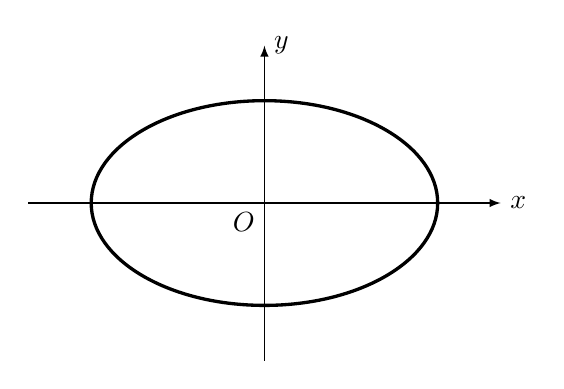
\begin{tikzpicture}[>=latex]
    \draw[->](-3,0)--(3,0)node[right]{$x$};
\draw[->](0,-2)--(0,2)node[right]{$y$};
\node at (0,0) [below left]{$O$};
\draw[very thick](0,0) ellipse [x radius=2.2, y radius=1.3];

\end{tikzpicture}
    \caption{}
\end{figure}

\begin{solution}
由于图形的对称性,只要求出椭圆在第一象限内的面积,再乘以4就是该椭圆的面积,所以
\[\frac{A}{4}=\int^a_0 y\dd x\]
这里将椭圆用参数方程
$\begin{cases}
    x=a\cos t\\ y=b\sin t
\end{cases}$
表出,当$x=a$时,$t=\arccos 1=0$; 当$x=0$时,$t=\arccos 0=\frac{\pi}{2}$, 于是
\[\begin{split}
    \frac{A}{4}=\int^0_{\tfrac{\pi}{2}}b\sin t \dd(a\cos t)&=\int^0_{\tfrac{\pi}{2}}(b\sin t )(-a\sin t)\dd t\\
&=ab \int^{\tfrac{\pi}{2}}_0 \sin^2 t\dd t=\frac{1}{4}ab\pi 
\end{split}\]
所以:$A=\pi ab$.
\end{solution}

\begin{ex}
\begin{enumerate}
    \item 求在曲线$y=\sin2x$, $y=0$, $x\in[0, 2\pi]$之间的面积.
    \item 求下列曲线所围图形的面积:
\begin{enumerate}
    \item $y=8-\frac{1}{2}x^2$和$y=3.2$ 
    \item $y=x^2-5x+7$和$y=-2x^2+10x-5$
    \item $y=\sin x$和$y=\frac{2}{\pi} x,\; x\ge 0$
\end{enumerate}
\item 求以曲线$y=\sin x\; \left(0\le x\le \frac{\pi}{4}\right)$;$y=\cos x\; \left(\frac{\pi}{4}\le x\le \frac{\pi}{2}\right)$和$y=0$为边界的区域的面积.

\item \begin{enumerate}
    \item 证明点$x=t^2-1$, $y=t(t^2-1)$在曲线$y^2=x^2(x+1)$上;
    \item 当$t$由$t=-2$变化到$t=2$时,作出曲线$\begin{cases}
        x=t^2-1\\x=t (t^2-1)
    \end{cases}$的图象;
\item 求由曲线的环路所围区域的面积.
\end{enumerate}

\item 在曲线$y=x^2-2x+2$与过点$(2, 3)$的直线所围的图形
中,求图形面积最小时的直线方程.
\item 求抛物线$y=x^2$及过此抛物线上点$(2, 4)$的切线和$x$轴所围图形的面积.
\item 已知曲线$C:\; y=x^2-7x+10\; (x>0)$与点$A(0, 1)$, 
回答下列问题:
\begin{enumerate}
    \item 求过点$A$所引曲线$C$的切线方程以及切点$T$的坐标.
    \item 设$S$是直线$x=1$与曲线$C$的交点.若曲线$C$上的动点$P$从$S$点运动到$T$点时,将线段$AP$所在的区域用阴影表示出来,并求出这个区域的面积.
\end{enumerate}

\item 求通过$(0, 0)$, $(1, 2)$两点的抛物线,要求它具有以
下的性质:
\begin{enumerate}
    \item 它的对称轴平行于$y$轴,且凸向上,
    \item 它与$x$轴所围区域的面积最小.
\end{enumerate}

\item 对称轴平行$y$轴的抛物线与圆$x^2+y^2=4$切于$A(0, 2)$点并通过$B(-2, 0)$点,计算抛物线与圆所围区域的面积.
\end{enumerate}
\end{ex}

\subsection{利用横断面算体积法}
对于空间的一个立体,我们取一条直线作为坐标轴,取直线上一点作为原点(图4.11),假定这立体紧夹于在$x=a$与$x=b$两点所作的$x$轴的垂直平面之间,又如果在离原点$x$处作这轴的一个垂直平面,并且该垂直平面截得立体的截面的面积是$x$的连续函数$A(x),\; a\le x\le b$, 那么立体的体积可由定积分来计算:
\begin{figure}[htp]
    \centering
\begin{tikzpicture}[>=latex]
    \draw[->](-.5,0)--(6,0)node[right]{$x$};
\tkzDefPoints{.8/0/a, 2/0/A, 3.3/0/x_i, 5/0/b, 0/0/O}
\tkzDrawPoints(a,A,x_i,b,O)
\tkzLabelPoints[below](a,x_i,b,O)
\tkzLabelPoint[below](A){$x_{i-1}$}
\node at (0,0){};
\draw[line width = 1pt] plot[smooth] coordinates{(.8,0)(1.2,.8)(2,1.3)(3.3,1.15)(5,0)(3.3,-1.15)(2,-1.3)(1.2,-.8)(.8,0)
};
\draw[dashed](A) ellipse [x radius=.35, y radius=1.3]; 
\draw[dashed](x_i) ellipse [x radius=.3, y radius=1.15]; 
\draw[thick](2,1.3) arc [start angle =90, end angle =270, x radius=.35, y radius=1.3];
\draw[thick](3.3,1.15) arc [start angle =90, end angle =270, x radius=.3, y radius=1.15];

\end{tikzpicture}
    \caption{}
\end{figure}

\begin{enumerate}
    \item 分$[a,b]$为$n$份,其分点
\[a=x_0<x_1<x_2<\cdots<x_n=b\]
    记$\|P_n\|=\max(x_i-x_{i-1})\quad i=1, 2,\ldots,n$.

    以平面$x=x_i,\; i=0, 1, 2,\ldots,n$截此立体为$n$个小单元,于是整个体积被看作这$n$个小单元的和.
\item  求阶梯函数的总和作为所求立体体积的近似和.考虑这样一个单元,它介于两个截面$x=x_{i-1},x=x_i$之间,于是以$(x_i-x_{i-1})$为高,以$A(x_{i-1})$作为底面积的直棱柱的体积是
  \[  A (x_{i-1}) (x_i-x_{i-1})\]
    于是,我们得到所求的体积$V$的近似表达式
    \[\sum^n_{i=1}A (x_{i-1}) (x_i-x_{i-1})\] 
    \item 对和取极限:当断面无限增加,$\|P_n\|\to 0$时,有
\[V=\lim_{n\to\infty}\sum^n_{i=1}A (x_{i-1}) (x_i-x_{i-1})=\int^b_a A(x)\dd x\]
\end{enumerate}

现在将上面的讨论总结为下面的定理.

\begin{blk}
   {定理} 如果已知一个给定的立体的垂直于一定方向所有的横断面的面积,取这些横断面的垂直方向作为$x$轴的方向,则这立体的体积由公式
\[V=\int^b_a A (x) \dd x\]
表达.其中$A(x)$是横坐标为$x$的横断面的面积,$a$、$b$为这立体的两端断面的横坐标. 
\end{blk}

\begin{example}
    求底边长为$a$, 高为$h$的正四棱锥的体积.
\end{example}

\begin{figure}[htp]
    \centering
\begin{tikzpicture}[>=latex]
    \tkzDefPoints{0/0/A, 3/0/B, 4/1/C}
    \tkzDefPointsBy[translation= from B to C](A){D}
    \tkzInterLL(A,C)(B,D)  \tkzGetPoint{O}
    \tkzDefPoints{0/3.5/E, 5/3.5/F}
    \tkzDefPointBy[projection = onto E--F](O) \tkzGetPoint{OO}
    \draw[|<->|](.7,1.4)--node[fill=white]{$y$}(2.7,1.4);
    \tkzDrawSegments(OO,A OO,B OO,C A,B B,C)
    \tkzDrawSegments[dashed](OO,D OO,O C,D D,A)
    
    \foreach \x in {A,B,C,D,O}
    {
        \tkzDefPointWith[linear, K=.66](OO,\x)  \tkzGetPoint{\x'}
        \tkzDefPointWith[linear, K=.33](OO,\x)  \tkzGetPoint{\x''}
    }
    \tkzDrawSegments(A',B' B',C' A'',B'' B'',C'')
    \tkzDrawSegments[dashed](C',D' D',A' C'',D'' D'',A'')
\draw[->](OO)--(2,4)node[right]{$x$};
\draw(-1,3.5)--(5,3.5);
\draw[dashed](.2,.5)--(O);
\draw(-1,0.5)--(.2,.5);
\draw[<->](-.8,0.5)--node[fill=white]{$h$}(-.8,3.5);
\draw[<->](4.8,0.5)--node[fill=white]{$x$}(4.8,1.5);
\draw[<->](4.8,1.5)--node[fill=white]{$h-x$}(4.8,3.5);
\draw[<->](3.8,1.5)--node[fill=white]{$\Delta x$}(3.8,2.5);
\tkzDefMidPoint(B,C) \tkzGetPoint{G}
\tkzDefMidPoint(B',C') \tkzGetPoint{G'}
\tkzDefMidPoint(B'',C'') \tkzGetPoint{G''}
\tkzDrawSegments[dashed](O,G O',G' O'',G'')
\tkzDefPointWith[linear, K=2](O,G) \tkzGetPoint{H}
\tkzDefPointWith[linear, K=3](O',G') \tkzGetPoint{H'}
\tkzDefPointWith[linear, K=4.5](O'',G'') \tkzGetPoint{H''}
\tkzDrawSegments(G,H G',H' G'',H'')
\tkzLabelPoints[below](O)

\draw[|<->|](0,-0.25)--node[fill=white]{$a$}(3,-.25);


\end{tikzpicture}
    \caption{}
\end{figure}

\begin{solution}
    设$x$为从底面到截面的距离,$y$为截面正方形的边长(图4.12),于是
\[\frac{h-x}{h}=\frac{y}{a}\]
即:$y=\frac{a}{h}(h-x)$.

截面面积
\[A(x)=\frac{a^2}{h^2}(h-x)^2\]
所以
\[\begin{split}
    V&=\int^h_0 \left(\frac{a}{h}\right)^2(h-x)^2 \dd x\\
    &=-\left(\frac{a}{h}\right)^2\frac{(h-x)^3}{3}\Bigg|^h_0=\frac{1}{3}a^2 h
\end{split}\]
\end{solution}

如果立体是一个旋转体,即先给出一条平面曲线
$y=f(x)$, 绕$x$轴旋转所得出的立体,我们的横断面就是以$y$为半径的圆,所以这立体的体积就等于
\[V=\pi \int^b_a y^2\dd x\]
如果$c\le y\le d$,$x=g(y)$绕$y$轴旋转,则
\[V=\pi \int^d_c x^2\dd y\]


\begin{example}
若球的半径是$a$, 球缺的高是$h$, 求球缺的体积.
\end{example}

\begin{figure}[htp]
    \centering
\begin{tikzpicture}[>=latex, scale=1.5]
    \draw[->](-1.5,0)--(2,0)node[right]{$x$};
    \draw[->](0,-1.5)--(0,1.5)node[right]{$y$};
    \draw[very thick](0,0)circle(1);
\draw(.4,1)--(.4,-1.5);
\draw(1,0)--(1,-1.5);
\draw[<->](0,-1.3)--node[below]{$a-h$}(.4,-1.3);
\draw[<->](0.4,-1.1)--node[fill=white]{$h$}(1,-1.1);
\draw[<->](-.2,0)--node[fill=white]{$a$}(-.2,1);

\draw[pattern=north east lines](45:1) arc (45:50:1)--(.64,0)--(1/1.414,0)--(45:1);
\draw[<->](0,1.3)--node[below]{$x$}(.64,1.3);
\draw(.64,1.5)--(.64,0);
\end{tikzpicture}
    \caption{}
\end{figure}


\begin{solution}
球是由圆$x^2+y^2=a^2$绕$x$轴旋转所得到的立体,且球心到球缺底面的距离为$a-h$, 设球心到截面的距离为$x$, 则截面圆的面积$A (x) =\pi y^2=\pi  (a^2-x^2)$.(图4.13)

所以
\[\begin{split}
    V=\pi\int^a_{a-h}(a^2-x^2)\dd x&=\pi\left[a^2 x-\frac{1}{3}x^3\right]\Bigg|^a_{a-h}\\
    &=\frac{\pi h^2}{3}(3a-h)
\end{split} \]
\end{solution}

\begin{example}
    计算底面半径分别为$r$和$R$, 高为$h$的圆台体积$V$.
\end{example}

\begin{solution}
此圆台可看作$xy$平面上的直线段
\[y=\frac{R-r}{h}x+r,\; (0\le x\le h),\quad x=0,\quad x=h,\quad y=0\]
所围成的直角梯形绕$x$轴旋转所得到的立体,从而
\[\begin{split}
    V&=\pi\int^h_0 \left(\frac{R-r}{h}x+r\right)^2 \dd x\\
    &=\pi\left[\left(\frac{R-r}{h}\right)^2\frac{x^3}{3}+2r\cdot \frac{R-r}{h}\cdot \frac{x^2}{2}+r^2 x\right]\Bigg|^h_0\\
    &=\frac{\pi h}{3}(R^2+Rr+r^2)
\end{split}\]
\end{solution}

\begin{example}
在第一象限中,由$y=\frac{x}{1-x}\; (x\ne 1)$, $y=1$, $y=0$和$x=1$所围成的图形绕着直线$x=1$旋转,求所生成的旋转体的体积(图4.14).
\end{example}

\begin{figure}[htp]
    \centering
\begin{tikzpicture}[>=latex, scale=2.5]
    \draw[->](-.25,0)--(1.8,0)node[right]{$x$};
    \draw[->](0,-.25)--(0,1.8)node[right]{$y$};
\draw[domain=0:.6, samples=100, very thick]plot(\x, {\x/(1-\x)});
\draw(1,0)node[below]{1}--(1,1.5)node[above]{$x=1$};
\draw[dashed](0,1)node[left]{1}--(1,1);
\draw[domain=0:.5, samples=100, pattern=north east lines]plot(\x, {\x/(1-\x)})--(1,1)--(1,0)--(0,0);

\draw[<->|](1.1,0)--node[fill=white]{$y$}(1.1,.4);
\draw[domain=0.286:.333, samples=10, pattern=north west lines]plot(\x, {\x/(1-\x)})--(1,.5)--(1,0.4)--(0.286,0.4);
\draw[|<->|](0.286,0.25)--node[fill=white]{$1-x$}(1,.25);

\end{tikzpicture}
    \caption{}
\end{figure}

\begin{solution}
$y$轴垂直于旋转体的横断面,设原点到横断面的距离为$y$, 则该横断面的面积
\[A (y) =\pi  (1-x)^2\]
由于函数$y=\frac{x}{1-x}$是单射的,故反函数存在,由它解出
\[x=\frac{y}{1+y},\qquad 1-x=\frac{1}{1+y}\]
于是
\[A(y)=\frac{\pi}{(1+y)^2}\]
\[\begin{split}
    V=\int^1_0 A(y)\dd y&=\pi\int^1_0 \frac{\dd y}{(1+y)^2}\\
&=-\pi\left(\frac{1}{1+y}\right)\Bigg|^1_0=-\pi\left(\frac{1}{2}-1\right)=\frac{\pi}{2}
\end{split}\]
\end{solution}

\begin{figure}[htp]
    \centering
    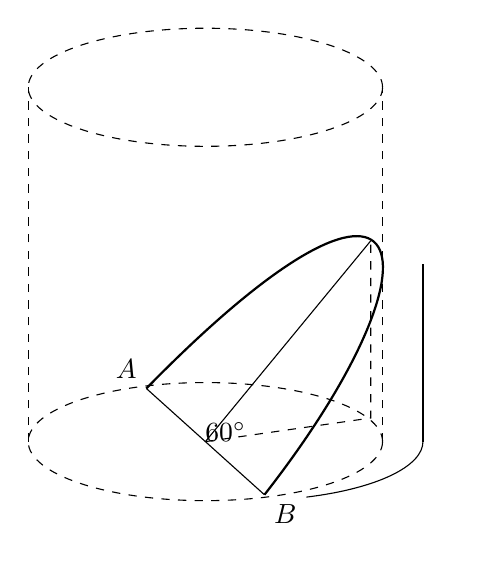
\begin{tikzpicture}[>=latex, scale=1.5]
\draw[dashed](0,0) ellipse [x radius=1.5, y radius=.5];
\draw[dashed](0,3) ellipse [x radius=1.5, y radius=.5];
\draw[dashed](-1.5,0)--(-1.5,3);
\draw[dashed](1.5,0)--(1.5,3);
\draw(.5,-.45)node[below right]{$B$}--(-.5,.45)node[above left]{$A$};
\draw[thick] (-.5,.45) .. controls (1.8,2.8) and (2.1,1.6) .. (.5,-.45);
\draw(0,0)--(1.4,1.7);
\draw[dashed](0,0)--(1.4,.2)--(1.4,1.7);
\tkzDefPoints{0/0/O, 1.4/.2/B1, 1.4/1.7/C}
\tkzMarkAngle[mark=none, size=.4, ->](B1,O,C)
\tkzLabelAngle[pos=.6](B1,O,C){$60^{\circ}$}
\tkzLabelPoints[left](O)
\draw(1.5,0) arc [start angle = 0, end angle =-70, x radius=1.5, y radius=.5];
\draw(1.5,0)--(1.5,1.5);
    \end{tikzpicture}    
    \caption{}
\end{figure}

\begin{ex}
\begin{enumerate}
    \item 底面半径为$a$的直圆柱,用通过底面一条直径并与底面成$60^{\circ}$角的平面去
    截,得到图4.15的立体,求其体积.
    \item 由抛物线$y^2=4ax$和直线$x=h$所围成
    的区域绕$x$轴旋转一周,求所生成旋转体的体积.
    \item 求底面半径为$r$, 高为$h$的圆锥体的
    体积.
    \item 设由椭圆$\frac{x^2}{a^2}+\frac{y^2}{b^2}=1$所围成的区域绕$x$轴旋转,求此旋转
    椭圆体的体积.
    \item 由曲线$y=\frac{\ln x}{x}$, $x$轴和通过曲线的最高点的纵坐标所围
    成的区域绕$x$轴旋转,求该旋转体的体积.
    \item 两条抛物线有公共的顶点和公共的对称轴,但位于两个
    互相垂直的平面内,一个运动着的椭圆,其中心在两抛物线的公共轴上,它的平面与公共轴垂直,它的顶点位于两条抛物线上,如果椭圆从公共顶点开始,移动一段距离$h$, 求由此椭圆所生成的体积.
    \item 求$y=4-x^2$与$x$轴之间的区域绕直线$y=-1$一周所生成的体积.
    \item 求圆$x^2+(y-b)^2=a^2\; (0<a<b)$绕$x$轴旋转所生成的旋转体的体积.
\end{enumerate}
\end{ex}

\section{简单初值问题{}---{}不定积分的简单应用}

在本章第2节,我们曾说过,一个函数的原函数有无穷多个,它们彼此之间相差一个常数.但是,在许多问题中,我们感兴趣的往往并不是这无穷多个原函数的全体(不定积分),而是某一个特定的原函数,在几何上,就是一条特定的积分曲线.为了求得这条积分曲线,必须知道它所经过的一个点,也就是说,要知道初始条件,在实际问题中,求满足一定初始条件的原函数问题是很多的,下面举一些简单的实例.

\begin{example}
    已知一质点$m$作具有匀加速度$a$的直线运动,设它的初速度为$u$, 求质点在$t$秒后所经过的距离.
\end{example}

\begin{solution}
由于$\frac{\dd v}{\dd t}=a$,所以
\begin{equation}
    v=at+C
\end{equation}
因为,当$t=0$时,$v=u$,代入(4.24)得:$C=u$,所以
\begin{equation}
    v=at+u
\end{equation}
由于$\frac{\dd s}{\dd t}=u+at$,分离变量,把它写成
\[\dd s=(u+at)\dd t\]
两边求不定积分,得
\[\int \dd s=\int (u+at)\dd t\]
\begin{equation}
    s=ut+\frac{1}{2}at^2+C'
\end{equation}
由初始条件:当$t=0$时,$s=0$,代入(4.26),得:$C'=0$,所以
\begin{equation}
    s=ut+\frac{1}{2}at^2
\end{equation}
为所求.(4.25)和(4.27)就是我们常见的运动学公式.
\end{solution}


\begin{example}
假设在原点处斜抛一质点$m$, 它的初速度$v_0$与水平$x$轴成$\alpha$角,又作用在质点$m$上的力只有向下的重力,求质点$m$的轨迹方程.
\end{example}

\begin{solution}
    设质点$m$的坐标是$(x,y)$,它的质量为$M$克,于是沿着$x$轴和$y$轴的速度分量分别是
    \[v_x=\frac{\dd x}{\dd t},\qquad v_y=\frac{\dd y}{\dd t}.\]
    而沿着$x$轴和$y$轴的加速度分量分别是
    \[\frac{\dd v_x}{\dd t}=\frac{\dd^2 x}{\dd t^2},\qquad \frac{\dd v_y}{\dd t}=\frac{\dd^2 y}{\dd t^2}.\]
    根据牛顿第二定律,得到
\[
\begin{cases}
    M\frac{\dd v_x}{\dd t}=0\\
    M\frac{\dd v_y}{\dd t}=-Mg
\end{cases}
\]
即:
\[\begin{cases}
    \dd v_x=0\\ 
    \dd v_y=-g\dd t
\end{cases}\]
所以
%\begin{align}
\[
\begin{cases}
    v_x=C_1\\ 
    v_y=-gt+C_2
\end{cases}
\] %\end{align}
常数$C_1$和$C_2$由初始条件决定,所以
\[ %\begin{align}
\begin{cases}
v_x=\frac{\dd x}{\dd t}=v_0\cos\alpha\\
v_y=\frac{\dd y}{\dd t}=-gt+v_0\sin\alpha
\end{cases}
\] 
即:
\[\begin{cases}
    \dd x=v_0\cos\alpha \dd t\\ \dd y=(-g t+v_0\sin\alpha)\dd t
\end{cases}\]
再求不定积分得
\[\begin{cases}
    x=(v_0\cos\alpha)t+C_3\\
    y=-\frac{gt^2}{2}+(v_0\sin\alpha)t+C_4
\end{cases}\]
由于,当$t=0$时,$x=y=0$,因此:
\[C_3=C_4=0\]
于是得到质点$m$以时间$t$为参变数的轨迹方程
\begin{align}
\begin{cases}
    x=(v_0\cos\alpha)t\\
    y=-\frac{gt^2}{2}+(v_0\sin\alpha)t
\end{cases}
\end{align}
消去$t$,得:
\[y=\frac{-gx^2}{2v^2_0 \cos^2\alpha}+x\tan\alpha\]
化为标准式,得
\[\left(x-\frac{v^2_0\sin2\alpha}{2g}\right)^2=-\frac{2v^2_0\cos^2\alpha}{g}\left(y-\frac{v^2_0\sin^2\alpha}{2g}\right)\]
这是顶点在$\left(\frac{v^2_0\sin2\alpha}{2g},\frac{v^2_0\sin^2\alpha}{2g}\right)$处的抛物线方程(如图4.16),且从顶点到焦点的方向是$y$轴的负方向,又焦点到准线的距离是$\frac{v^2_0 \cos^2\alpha}{g}$,因此,从顶点到它的上方的准线距离等于$\frac{v^2_0 \cos^2\alpha}{2g}$,而准线到$x$轴的距离就等于
\[\frac{v^2_0 \cos^2\alpha}{2g}+\frac{v^2_0 \sin^2\alpha}{2g}=\frac{v^2_0}{2g}\]
故准线的位置仅依赖于初速度的大小,而与抛射角的大小无关.

\begin{figure}[htp]
    \centering
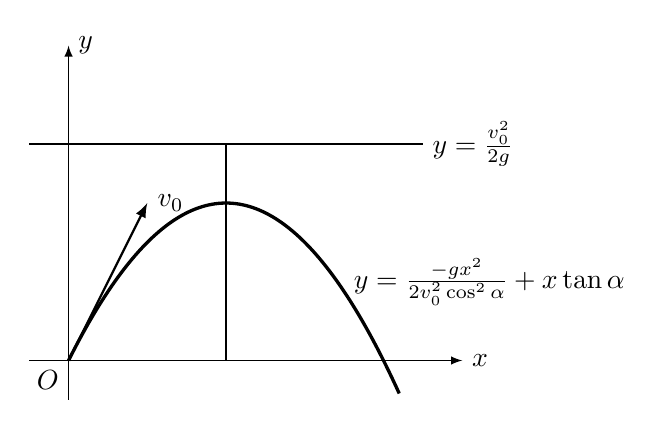
\begin{tikzpicture}[>=latex]
\draw[->](-.5,0)--(5,0)node[right]{$x$};
\draw[->](0,-.5)--(0,4)node[right]{$y$};
\draw[domain=0:4.2, samples=100, very thick]plot(\x, {0.5*(-\x*\x+4*\x)});
\draw(-.5,2.75)--(4.5,2.75)node[right]{$y=\frac{v^2_0}{2g}$};
\node at (3.5,1)[right]{$y=\frac{-gx^2}{2v^2_0 \cos^2\alpha}+x\tan\alpha$};
\node at (0,0)[below left]{$O$};
\draw(2,2.75)--(2,0);
\tkzDefPoints{2/2/A, 2/1.25/S}
\tkzDrawPoints(A,S)
\tkzLabelPoints[above right](A,S)
\draw[->, thick](0,0)--(1,2)node[right]{$v_0$};


\end{tikzpicture}
    \caption{}
\end{figure}
\end{solution}

下面我们来讨论人口的增长与放射性元素蜕变的问题.

在很多单纯的自然现象中,一个随着时间而变化的量$y(t)$的变化率常常和$y(t)$当时的值成正比例,用数学式表达,即存在一个随该现象而定的常数$k$(与$t$无关),使得
\[y' (t) =ky (t) \]
或
\begin{equation}
    \frac{\dd }{\dd t}y(t)=ky(t)
\end{equation}
人口的增长与放射性元素的蜕变就是这样的两个例子.

假如人口按某一固定的“增长率”$k$增长,譬如时间单位是“年”,增长率2\%, 则$k=2\%$. 设人口随时间变化的函数是$y(t)$, 本来$y(t)$是整数,但由于数量很大,我们可以把它看作一个平滑函数,$y(t)$满足下面的条件:
\[y(t+\Delta t)-y(t)=ky(t)\cdot \Delta t\]
换言之,人口增加数量与这段时间开始的人口数,以及这段时间间隔成比例,也即
\[\frac{y(t+\Delta t)-y(t)}{\Delta t}=ky(t)\]
令$\Delta t\to 0$, 由上式得到
\[\frac{\dd }{\dd t}y(t)=ky(t)\]
也就是说,人口在时刻$t$的瞬时变率与当时的值$y(x)$成正比例.为求出函数$y(t)$, 我们来解具有初始条件的微分方程
\begin{numcases}{}
    \frac{\dd }{\dd t}y(t)=ky(t)\\
    y(0)=A
\end{numcases}
将(4.33)改写成
\[\frac{\dd y(t)}{y(t)}=k\dd t\]
即:$\ln[y(t)]=kt+C$,由初始条件确定常数$C$的值,得:
\[\ln A=C\]
所以:$\ln[y(t)]=kt+\ln A$,
移项,得:
\[\ln\frac{y(t)}{A}=kt\]
由此得:
\[\frac{y(t)}{A}=e^{kt}\]
所以:$y(t)=Ae^{kt}$为所求.



总结上面的讨论,得到以下命题:

\begin{blk}{命题}
    设$y'(t)=ky(t)$,$y(0)=A$,则:
    \[y(t)=Ae^{kt}\]
\end{blk}




\begin{example}
    若某城市现有人口10万,按照每年3\%的比率增长,问几年后人口是现有人口的2倍?
\end{example}

\begin{solution}
    设$t_1$年后人口加倍,于是依题意有
\[10e^{3\%t_1}=2\x10\]
即:$e^{0.03t_1}=2$, 两边取常用对数,得
\[\begin{split}
    0.03t_1\lg e&=\lg2\\
t_1&= \frac{100\lg2}{3\lg e}\approx \frac{100}{3}\cdot\frac{0.3010}{0. 4343}\\
&\approx \frac{100}{3}\cdot 0.6931\approx 23.
\end{split} \]
答:约23年后,人口会加倍.
\end{solution}

从问题的解法看出,人口的加倍期仅与增长率有关,即$t_1=\frac{\ln2}{k}$, 下面是二者之间的对照表.

\begin{center}
\begin{tabular}{c|ccccc}
\hline
    增长率$k$ & 0.05&0.04&0.03&0.02&0.01\\
\hline
加倍期$t_1$ & 约14年& 约17年& 约23年& 约34.5年& 约39年\\
\hline
        \end{tabular}
\end{center}

同样地可把上述命题应用于放射性元素蜕变问题.

\begin{example}
    放射性元素的数量随时间$t$变化的函数是$N(t)$, $A=N(0)$是起算时的数量,$k$是蜕变率,且知放射性元素经过$\Delta t$这段时间的蜕变,它减少的数量$\Delta N(t)=N(t+\Delta t)-N(t)$与在时刻$t$的数量$N(t)$及这段蜕变时间$\Delta t$成比
例,即
\[\Delta N (t) =-kN (t) \cdot \Delta t\]
因为放射性元素不断减少,所以$\Delta N$是负数,问经过多少年放射性元素剩下了一半?
\end{example}

\begin{solution}
    依题意,有
\[\frac{\dd N}{\dd t}=-kN (t) \]
根据本节命题,得到
\[N (t) =Ae^{-kt}\]

设经过$t_1$年,放射性元素减少了一半,通常称$t_1$为放射性元素的半衰期,于是
\[t_1=\frac{\ln 2}{k}\approx \frac{0. 6931}{k}\]
\end{solution}

下面是一些放射性元素的半衰期的简表.

\begin{center}
    \begin{tabular}{c|ccc}
    \hline
        元素 & 氩Ar$^{39}$ &碳C$^{14}$&氢H$^3$  \\
    半衰期 & 269年& 5730年& 12.3年 \\
    \hline
    元素 & 碘I$^{129}$ &铀U$^{238}$& 铀U$^{235}$ \\
    半衰期 &  $16\x10^6$年& $4.5\x 10^9$年& $0.71\x 10^9$年\\
    \hline
            \end{tabular}
    \end{center}

我们可以把岩石或化石中所含的各种微量的放射性元素,当作天然的计时仪表,因为各种放射性元素的微量都可以测量十分准确,所以我们可以通过对残留微量的测定,
用半衰期去推算岩石或化石的“年龄”,甚至于我们所居住的地球的“年龄”.

\begin{ex}
\begin{enumerate}
    \item 求下列积分曲线:
\begin{multicols}{2}
\begin{enumerate}
    \item $\begin{cases}
        y'=2x\\
        y|_{x=x_0}=y_0
    \end{cases}$
    \item $\begin{cases}
        y'=2\sqrt{y}\\
        y|_{x=0}=0
    \end{cases}$
    \item $\begin{cases}
        y'=\frac{2}{3\sqrt[3]{x}}\\
        y|_{x=0}=4
    \end{cases}$
\end{enumerate}
\end{multicols}
\item 在$20.2^{\circ}{\rm C}$, 细菌受到5\%的消毒溶液消毒,每小时细菌死
    亡的比率为11\%, 假如开始时有1000个细菌,那么在24小时后还剩下多少?
    \item 化学反应速度$v$和温度$t$的增加是按照有机体生长的规律
    进行的,当$t=0$时,$v=30$; 当$t=9.90$时,$v=60$, 求反应率以及当$t=20$时,$v$的值.
\item 若函数$y=f(x)$的变率$\frac{\dd y}{\dd x}$与当时的函数值的平方成
    正比例,且当$x=0$时,$y=f(0)=2$; 当$x=1$时,$y=f(1)=4$, 求函数$y=f(x)$.
\end{enumerate} 
\end{ex}

\subsection*{习题4.5}
\begin{enumerate}
    \item 计算下列不定积分:
\begin{multicols}{2}
\begin{enumerate}
    \item $\displaystyle\int \frac{\dd x}{1-3x^2}$
    \item $\displaystyle\int \frac{1-\sin^{-3}x}{1-\cos^2 x}\dd x$
    \item $\displaystyle\int \frac{\dd x}{\sin x\cos x}$
    \item $\displaystyle\int x\sec^2 x\dd x$
    \item $\displaystyle\int xe^{2x+1}\dd x$
    \item $\displaystyle\int \frac{x^2+2}{x(x-1)}\dd x$
\end{enumerate}
\end{multicols}

\item 求下列定积分:
\begin{multicols}{2}
    \begin{enumerate}
        \item  $\displaystyle\int_{-1}^{3} \frac{\dd x}{x^{2}+7 x+10} $
        \item  $\displaystyle\int_{\sqrt{3}}^{0} \frac{\dd x}{2+x^{2}}$
        \item  $\displaystyle\int_{0}^{1} x \sqrt{\left(2-x^{2}\right)^{3}} \dd x$
        \item  $\displaystyle\int_{0}^{\ln 3} \frac{\dd x}{e^{x}+5+6 e^{-x}}$
        \item  $\displaystyle\int_{1}^{\tfrac{7}{5}} \frac{x^{\tfrac{3}{4}}+x^{\tfrac{1}{4}}}{x^{\tfrac{9}{4}}-x^{\tfrac{5}{4}}+x^{\tfrac{1}{4}}} \dd x$
        \item  $\displaystyle\int_{1}^{2} \frac{2-x+x^{2}}{(1+x)(1-x)^{2}} \dd x$
        \item  $\displaystyle\int_{1}^{2} x \ln x \dd x$
        \item  $\displaystyle\int_{-\pi}^{\pi} \sin m x \sin n x \dd x$
        (此处 $m, n$ 是整数且 $m \pm n\ne 0$)
\item  $\displaystyle\int_{\tfrac{a}{\sqrt{3}}}^{a} \frac{\dd x}{\left(a^{2}+x^{2}\right)^{3 / 2}}$
\end{enumerate}
\end{multicols}
\item  求下列极限:
    \begin{enumerate}
\item  $\displaystyle\lim _{n \to  \infty} \frac{1}{n}\left\{\left(1+
\frac{1}{n}\right)^2+\left(1+\frac{2}{n}\right)^2+\cdots+
\left(1+\frac{n}{n}\right)^{2}\right\}$
\item $\displaystyle\lim _{n \to  \infty} \frac{1^{4}+2^{4}+\cdots+n^{4}}{n^{5}}$
\item $\Lim_{n\to\infty}\frac{1}{n}\left(\sin\frac{\pi}{n}+\sin\frac{2\pi}{n}+\cdots+\sin\frac{n\pi}{n}\right)$
\item $\Lim_{n\to\infty}\left(\frac{1}{\sqrt{n+1}}+\frac{1}{\sqrt{n+2}}+\cdots+\frac{1}{\sqrt{n+n}}\right)\cdot \frac{1}{\sqrt{n}}$
\end{enumerate}

\item 利用求$y=\frac{1}{x}$的定积分,证明
\[\ln(n+1)<1+\frac{1}{2}+\frac{1}{3}+\cdots+\frac{1}{n}<1+\ln n.\]
\item 设$0<a\le 1$,求证:
\[\int^a_0\frac{\dd x}{x^3+1}<\int^a_0\frac{\dd x}{x^4+1}. \]
\item 设$0\le x\le \frac{\pi}{4}$,利用不等式$0\le \sin x\le x$证明:
\[\frac{\pi}{4}<\int^{\pi/4}_0\frac{\dd x}{\sqrt{1-\sin x}}<2-\sqrt{4-\pi}.\]

\item 若$m,n$是正整数,求证:
\[\int^1_0 x^m (1-x)^n\dd x=\frac{n}{m+1}\int^1_0x^{m+1}(1-x)^{n-1}\dd x. \]
\item 求证:$\displaystyle\int^\pi_0 xf(\sin x)\dd x=\frac{\pi}{2}\int^\pi_0f(\sin x)\dd x$.
\item 若$I_n=\displaystyle\int^{\pi/4}_0 \tan^n \theta \dd \theta\quad (n\ge 2)$. 试求$I_n$和$I_{n-2}$的关系式.
\item 若$I_n=\displaystyle\int \frac{\dd x}{(x^2+a^2)^n}$,求证:
\[2na^2I_{n+1}=\frac{x}{(x^2+a^2)^n}+(2n-1)I_n\]
\item 设$S_n=\frac{1}{\sqrt{1}}+\frac{1}{\sqrt{2}}+\cdots+\frac{1}{\sqrt{n}}$,$n$为正整数.
\[T_n=\frac{1}{\sqrt{1+\frac{1}{2}}}+\frac{1}{\sqrt{2+\frac{1}{2}}}+\cdots+\frac{1}{\sqrt{n+\frac{1}{2}}}.\]
求证:
\begin{multicols}{2}
\begin{enumerate}
    \item $S_n\ge \displaystyle\int^{n+1}_1 \frac{\dd x}{\sqrt{x}}$
    \item $\Lim_{n\to\infty}\frac{1}{S_n}=0$
    \item $S_{n+1}-1\le T_n\le S_n$
    \item $\Lim_{n\to\infty}\frac{T_n}{S_n}=1$
\end{enumerate}
\end{multicols}

\item 设$f(x)=(ax+b)e^{x/2}$, 求$a,b$的值,使得等式
\[f (x) =e^{x/2}-1+\frac{1}{2}\int^x_0 f (t) \dd t\]
对于任何$x$的值都成立.
\item 求由曲线$y=\frac{4}{x^2}$, $y=x-1$, $x=1$所围区域的面积.
\item 求在曲线$x^2+y^2=9$和$y=\frac{1}{3}(-x^2+1)$之间位于
第二象限那部分的面积.
\item 求积分$I(a)=\displaystyle\int^1_{-1}|x-a|e^x\dd x$在$|a|\le 1$时的最大值.
\item 设$0<t<\pi$,考察$x$的函数$f(x)=2\sin x\sin(t-x)$
\begin{enumerate}
    \item 画出$f(x)$在区间$0\le x\le \pi$上的图象,再设
    \[F (t) =\int^\pi_0 |f (x)|\dd x.\]
根据所作的图象说明$F(t)$所表示的是什么?
\item 用关于$t$的式子写出$F(t)$, 并求出使$F(t)$取最小值时$t$的值.
\end{enumerate}
\item  设$T_1$是由抛物线$y=4x^2$和直线$x=a$, $x=1$, $y=0$所
围成的区域,$T_2$是抛物线$y=4x^2$和二直线$x=a$, $y=0$围成的区域,但是$0<a<1$,试求:
\begin{enumerate}
\item $T_1$绕$x$轴旋转而成的旋转体体积$V_1$;    \item $T_2$绕$y$轴旋转而成的旋转体体积$V_2$;    \item 使$V_1+V_2$为最大时$a$的值.
\end{enumerate}
\item 设$0\le t\le \frac{\pi}{2}$,曲线$y=\sin x$与三条直线$x=t$, $x=2t$, 
$y=0$围成部分绕$x$轴旋转所成的旋转体的体积为$V(t)$.当$t=\alpha$时$V(t)$最大,试求$\cos\alpha$的值.
\item 设曲线$y=f(x)$通过点$P(3, 4)$, 并满足微分方程
$\frac{\dd y}{\dd x}=\frac{y}{x}$,
求此积分曲线.

\item 若$\frac{\dd y}{\dd x}=\cos(x+y)$,求不定积分.(提示:设$z=x+y$)
\end{enumerate}
